\documentclass[10pt,notitlepage]{book}

\usepackage{preambulle}
\usepackage[Rejne]{fncychap}
\fancyhead[L]{\scriptsize Nora \textsc{Nicolas} \& Jérémy \textsc{Auffinger}}
\fancyhead[R]{\scriptsize \textsc{UE PG -- Fiche de travaux dirigés}}

\titleformat{\section}{\color{blue}\bfseries\large}{\hspace{-0.3em}
Exercice~\arabic{section})}{.2em}{}{}
\titleformat{\subsection}{\color{brandeisblue}\bfseries}{\hspace{-0.3em}
\arabic{section}) \arabic{subsection}-}{.5em}{}{}
\titleformat{\subsubsection}{\color{capri}\bfseries}{\hspace{-0.3em}
\arabic{section}) \arabic{subsection}- \alph{subsubsection}.}{.5em}{}{}

\newlength\tindent
\setlength{\tindent}{\parindent}
\setlength{\parindent}{0pt}
\renewcommand{\indent}{\hspace*{\tindent}}

\begin{document}

\begin{center}
\Huge Physique générale : Optique\smallbreak\vspace*{-14pt}
\rule[11pt]{5cm}{0.5pt}\smallbreak\vspace*{-14pt}
\huge Chapitres 1 à 4
\end{center}

\toccontents

\setcounter{chapter}{-1}
\chapter{Conseils généraux}
\vspace*{-55pt}
Ce document à pour but de rappeler et résumer les conseils, arguments et astuces
qui ont pu être vues et énoncées durant les TDs. Il ne remplace ni les séances
en elles-mêmes, où votre participation active est nécessaire (c'est en se
trompant qu'on sait comment ne pas faire, et donc comment bien faire), ni les CM
de votre professeur-e. J'espère néanmoins qu'il saura vous être utile.
\smallbreak

La première partie comporte quelques éléments généraux sur l'optique. D'autres
conseils et éléments importants sont mis en valeur quand ils sont pertinents :
le code couleur reste le même, dans le but d'avoir une structure facilement
navigable. Les bases de réflexion, données ou définitions, sont en vert. Les
résultats importants, propriétés ou résultats à trouver, sont en rouge. Les
points pivots de réflexion, démonstration ou outils à choisir judicieusement,
sont en bleu. Les côtés pratiques, exemples et applications, sont en gris.
\smallbreak

Les premiers exercice du chapitre 1 sont intégralement corrigés, et certains
mots importants (comme « divergent ») ont une note de fin du chapitre 1 avec une
brève définition. Ces exercices représentent la base de comment construire sa
réflexion face à un exercice de pĥysique (d'optique particulièrement), mais ils
ne sont pas tous corrigés ainsi. Ainsi, vous verrez qu'après quelques exemples,
je vous renvoie aux corrigés que vous avez à disposition sur \textit{Claroline}.
Les schémas y sont clairs et j'espère que ma retranscription écrite du
raisonnement derrière ces schémas suffiront à vous guider. \hfill Bonne lecture,
\smallbreak

Nora \textsc{Nicolas} --
\href{mailto:n.nicolas@ip2i.in2p3.fr}{n.nicolas@ip2i.in2p3.fr}\\
Jérémy \textsc{Auffinger} --
\href{mailto:j.auffinger@ip2i.in2p3.fr}{j.auffinger@ip2i.in2p3.fr}\\

\begin{NCprop}{Principe des exercices de physique}
    Tout exercice de physique suit le schéma suivant :
    \begin{enumerate}
        \item Lecture de l'énoncé en français et relevé des données ;
        \item Traduction des données en schéma si pertinent, et en expression
            mathématique si pertinent ;
        \item Compréhension de la réponse attendue ;
        \item Traduction de la réponse attendue en schéma si pertinent, et en
            expression mathématique si pertinent ;
        \item Détermination d'un ou de plusieurs outils (relation mathématique,
            règle de construction...) du cours faisant le lien entre les données
            et la réponse : répéter si besoin d'une réponse intermédiaire ;
        \item Application.
    \end{enumerate}
    Un exemple est donné partie \ref{ssec:vp}.
\end{NCprop}


\begin{NCcoro}{Conseils}
    Avant d'encadrer un résultat :
    \begin{enumerate}
        \item Vérifer la cohérence mathématique avec la ligne précédente : les
            signes devant les grandeurs, le nombre de grandeurs, ne pas oublier
            les fonctions inverses... ;
        \item Vérifier l'homogénéité de part et d'autre de l'équation pour les
            résultats littéraux ;
        \item Vérifier la cohérence physique de la valeur numérique, notamment à
            l'aide d'un schéma.
    \end{enumerate}
\end{NCcoro}

\begin{NCimpo}{Important}
    L'erreur la plus simple mais la plus grave à faire est de se tromper sur une
    grandeur algébrique :
    \begin{center}
        \textbf{\underline{Toujours vérifier le sens des grandeurs algébriques}}
    \end{center}
\end{NCimpo}

\chapter{Lentilles minces}\label{ch:O1}
\vspace*{-24pt}

\begin{center}
    \Huge Exercices d'application
\end{center}

\section{Constructions optiques dans toutes les situations}
Pour construire une image à partir d'un objet, on utilise les règles de
construction :

\begin{defi}[label = rconst]{Règles de construction}
    \begin{enumerate}
        \item Tout rayon passant par le centre optique $O$ n'est pas dévié ;
        \item Tout rayon incident passant par le foyer objet $F$ de la lentille
            émerge parallèlement à l'axe optique ;
        \item Tout rayon indicent parallèle à l'axe optique émerge de la
            lentille en passant par le foyer image $F'$ de la lentille.
    \end{enumerate}
\end{defi}

\pagebreak

\begin{center}
    \huge Constructions pour une lentille convergente
\end{center}

\subsection{Objet à distance finie}
\subsubsection{Avant le foyer objet}
\begin{wrapfigure}[5]{R}{.45\linewidth}
    \vspace*{-20pt}
    \centering
    \begin{tikzpicture}[scale=0.9]
        % Axe optique
        \draw[thin,->](-3.5,0)--(3.5,0)node[below]{A.O.};
        % Lentille
        \coordinate (O) at (0,0);
        \def \fa{1.5};
        \def \lsiz{2};
        \coordinate (F) at ($(O)+(-\fa,0)$);
        \coordinate (Fp) at ($(O)+(\fa,0)$);
        
        \foreach \x/\z in {O/\fa}{
            \draw[shift={(\x)}] (0,0)
                node[below left] {O$_{}$};
            \draw[shift={(\x)}] (\z,2pt) --++ (0,-4pt)
                node[below right] {F$'_{}$};
            \draw[shift={(\x)}] ({-\z},2pt) --++ (0,-4pt)
                node[below right] {F$_{}$};}
        
        \draw[shift={(O)}, thick, <->, >=latex] (0,-\lsiz)--(0,\lsiz)
            node[above]{$\Lc_{}$};
        % Objet
        \def \pos{-3}
        \def \siz{1}
        \coordinate (A) at ($(O)+(\pos,0)$);
        \coordinate (B) at ($(A)+(0,\siz)$);
        \draw[->, Purple!70] (A) 
            node[below] {A}
            -- (B)
            node[above, left] {B};

        % Rayons pour objet avant foyer d'une lentille convergente
        \len{(A)}{(O)}{\posi}
        \len{(A)}{(B)}{\size}
        \len{(O)}{(F)}{\foc}
        \draw[brandeisblue, simple] (B) -- (O);
        \draw[orange!70, simple, name path=OBp] (O) --++ ($(O)-(B)$);
        \draw[brandeisblue, double] (B) --++ (\posi,0) coordinate (I);
        \def \mut{2}
        \draw[orange!70, double, name path=IBp] (I) --++ ($\mut*(Fp)-\mut*(I)$);
        \def \intsiz{\size*\foc/(\posi-\foc)}
        \draw[brandeisblue, triple] (B) -- (F)
            --++ (\foc,-{\intsiz}) coordinate (E);
        \def \mut{2}
        \draw[orange!70, triple, name path=EBp] (E) --++ (\mut*\foc,0);
        \path[name intersections={of=OBp and IBp, by=B\bp}];
        \coordinate (A\bp) at ($(B\bp)+(0,{\intsiz})$);
        \draw[->, Red!70] (A\bp) 
        node[above] {A\bp}
        -- (B\bp)
        node[below, right] {B\bp};
    \end{tikzpicture}
    \label{fig:convAF}
\end{wrapfigure}

On utilise aisément les règles sus-citées en traçant :
\begin{enumerate}
    \item Le rayon passant par $B$ et par $O$ : il ne sera pas dévié ;
    \item Le rayon passant par $B$ et parallèle à l'A.O. : il passe par $F'$ en
        sortie ;
    \item Le rayon passant par $B$ et par $F$ : il émerge parallèle à
        l'\ed{A.O.}{axe optique}.
\end{enumerate}

Ces rayons, issus d'un \underline{\ed{objet réel}{qui existe physiquement, situé avant
la face d'entrée du système optique}}, se croisent après la lentille :
on a un faisceau émergent \underline{\ed{convergent}{dont la prolongation dans
le sens positif de la marche des rayons mène à une
intersection}} qui donne une \underline{\ed{image réelle}{qui peut être
observée sur un support physique dans l'espace image du système, après la face
de sortie}}.

\subsubsection{Sur le foyer objet}
\begin{wrapfigure}[5]{R}{0.45\linewidth}
    \vspace*{-20pt}
    \begin{tikzpicture}[scale=1]
    % Axe optique
    \draw[thin, ->](-3,0)--(3,0)node[below]{A.O.};
    % Lentille 
    \coordinate (O) at (0,0);
    \def \fa{2}
    \def \lsiz{2}
    \coordinate (F) at ($(O)+(-\fa,0)$);
    \coordinate (Fp) at ($(O)+(\fa,0)$);

    \foreach \x/\z in {O/\fa}{
        \draw[shift={(\x)}] (0,0)
            node[below left] {O$_{}$};
        \draw[shift={(\x)}] (\z,2pt) --++ (0,-4pt)
            node[below right] {F$'_{}$};
        \draw[shift={(\x)}] ({-\z},2pt) --++ (0,-4pt)
            node[above right] {F$_{}$};
    }

    \draw[shift={(O)}, thick, <->, >=latex] (0,-\lsiz)--(0,\lsiz)
        node[above]{$\Lc_{}$};
    % Objet
    \def \pos{-2}
    \def \siz{1.5}
    \coordinate (A) at ($(O)+(\pos,0)$);
    \coordinate (B) at ($(A)+(0,\siz)$);
    \draw[->, Purple!70] (A) 
        node[below] {A}
        -- (B)
        node[above, left] {B};
    % Rayons pour objet sur le foyer d'une lentille convergente
    \len{(A)}{(O)}{\posi}
    \len{(A)}{(B)}{\size}
    \len{(O)}{(F)}{\foc}
    \draw[brandeisblue, simple] (B) -- (O);
    \draw[orange!70, simple, name path=OBp] (O) --++ ($(O)-(B)$);
    \draw[brandeisblue, double] (B) --++ (\posi,0) coordinate (I);
    \def \mut{2}
    \draw[orange!70, double, name path=IBp] (I) --++ ($\mut*(Fp)-\mut*(I)$);
    % ---------------------------------------------------------------------        
    \end{tikzpicture}
    \centering
    \label{fig:convBF}
\end{wrapfigure}

De la même manière, on trace :
\begin{enumerate}
    \item Le rayon passant par $B$ et par $O$ : il ne sera pas dévié ;
    \item Le rayon passant par $B$ et parallèle à l'A.O. : il passe par $F'$ en
        sortie ;
    \item Le rayon passant par $B$ et $F$ ne passe pas par le système optique,
        ce rayon est inutile.
\end{enumerate}
Ainsi, à partir d'un \underline{objet réel}, on obtient des rayons parallèles
qui donnent une \underline{image à l'infini}.

\subsubsection{Entre le foyer et la lentille}\label{eflc}

\begin{wrapfigure}[4]{R}{.45\linewidth}
    \centering
    \begin{tikzpicture}[scale=1]
        % Axe optique
        \draw[thin, ->](-3,0)--(3,0)node[below]{A.O.};
        % Lentille 
        \coordinate (O) at (0,0);
        \def \fa{2}
        \def \lsiz{2}
        \coordinate (F) at ($(O)+(-\fa,0)$);
        \coordinate (Fp) at ($(O)+(\fa,0)$);

        \foreach \x/\z in {O/\fa}{
            \draw[shift={(\x)}] (0,0)
                node[below left] {O$_{}$};
            \draw[shift={(\x)}] (\z,2pt) --++ (0,-4pt)
                node[below right] {F$'_{}$};
            \draw[shift={(\x)}] ({-\z},2pt) --++ (0,-4pt)
                node[below right] {F$_{}$};
        }

        \draw[shift={(O)}, thick, <->, >=latex] (0,-\lsiz)--(0,\lsiz)
            node[above]{$\Lc_{}$};
        % Objet
        \def \pos{-0.8}
        \def \siz{1}
        \coordinate (A) at ($(O)+(\pos,0)$);
        \coordinate (B) at ($(A)+(0,\siz)$);
        \draw[->, Purple!70] (A) 
            node[below] {A}
            -- (B)
            node[above, left] {B};
        % Rayons pour objet entre le foyer et le centre d'une lentille convergente
        \len{(A)}{(O)}{\posi}
        \len{(A)}{(B)}{\size}
        \len{(O)}{(F)}{\foc}
        \draw[brandeisblue, simple] (B) -- (O);
        \draw[orange!70, simple] (O) --++ ($(O)-(B)$);
        \def \mut{1.5}
        \draw[orange!70, simplerev,
            dashed, name path=OBp] (B) --++ ($\mut*(B)-\mut*(O)$);
        \draw[brandeisblue, double] (B) --++ (\posi,0) coordinate (I);
        \def \mut{1.3}
        \draw[orange!70, double] (I) --++ ($\mut*(Fp)-\mut*(I)$);
        \draw[orange!70, doublerev,
            dashed, name path=IBp] (I) --++ ($-\mut*(Fp)+\mut*(I)$);
        \def \intsiz{\size*\foc/(\posi-\foc)}
        \draw[brandeisblue, triple] (B) -- (F)
            --++ (\foc,-{\intsiz}) coordinate (E);
        \def \mut{1.3}
        \draw[orange!70, triple] (E) --++ (\mut*\foc,0);
        \draw[orange!70, triplerev,
            dashed, name path=EBp] (E) --++ (-\mut*\foc,0);
        \path[name intersections={of=OBp and IBp, by=B\bp}];
        \coordinate (A\bp) at ($(B\bp)+(0,{\intsiz})$);
        \draw[->, Red!70] (A\bp) 
        node[below] {A\bp}
        -- (B\bp)
        node[below, right] {B\bp};
    \end{tikzpicture}
    \label{fig:convCF}
\end{wrapfigure}

Tout pareil, on trace :
\begin{enumerate}
    \item Le rayon passant par $B$ et par $O$ : il ne sera pas dévié ;
    \item Le rayon passant par $B$ et parallèle à l'A.O. : il passe par $F'$ en
        sortie ;
    \item Le rayon passant par $B$ et par $F$ : il émerge parallèle à l'A.O.
\end{enumerate}

\subsubsection{Après la lentille}
\begin{wrapfigure}[5]{R}{0.45\linewidth}
    \centering
    \begin{tikzpicture}[scale=1]
        % Axe optique
        \draw[thin, ->](-3,0)--(3,0)node[below]{A.O.};
        % Lentille 
        \coordinate (O) at (0,0);
        \def \fa{2}
        \def \lsiz{2}
        \coordinate (F) at ($(O)+(-\fa,0)$);
        \coordinate (Fp) at ($(O)+(\fa,0)$);

        \foreach \x/\z in {O/\fa}{
            \draw[shift={(\x)}] (0,0)
                node[below left] {O$_{}$};
            \draw[shift={(\x)}] (\z,2pt) --++ (0,-4pt)
                node[below right] {F$'_{}$};
            \draw[shift={(\x)}] ({-\z},2pt) --++ (0,-4pt)
                node[below right] {F$_{}$};
        }

        \draw[shift={(O)}, thick, <->, >=latex] (0,-\lsiz)--(0,\lsiz)
            node[above]{$\Lc_{}$};
        % Objet
        \def \pos{1.5}
        \def \siz{1.5}
        \coordinate (A) at ($(O)+(\pos,0)$);
        \coordinate (B) at ($(A)+(0,\siz)$);
        \draw[->, Purple!70] (A) 
            node[below] {A}
            -- (B)
            node[above, right] {B};
        % Rayons pour objet virtuel d'une lentille convergente
        \len{(A)}{(O)}{\posi}
        \len{(A)}{(B)}{\size}
        \len{(O)}{(F)}{\foc}
        \draw[brandeisblue, simple] ($2*(O)-(B)$) -- (O);
        \def \mut{1.5}
        \draw[orange!70, simple, name path=OBp] (O) --++ ($\mut*(B)-\mut*(O)$);
        \def \mut{2}
        \draw[brandeisblue, double] ($(B)-(\mut*\posi,0)$)
            --++ (\mut*\posi-\posi,0) coordinate (I);
        \draw[brandeisblue, dashed, double] (I) --++ (2*\posi,0);
        \def \mut{1.2}
        \draw[orange!70, double, name path=IBp] (I) --++ ($\mut*(Fp)-\mut*(I)$);
        \def \intsiz{\size*\foc/(\posi+\foc)}
        \draw[brandeisblue, triple] (F) --++ (\foc,{\intsiz}) coordinate (E);
        \def \mut{1.2}
        \draw[brandeisblue, dashed, triple] (E) -- (B) --++ ($\mut*(B)-\mut*(E)$);
        \draw[orange!70, triple, name path=EBp] (E) --++ (1.5*\posi,0);
        \path[name intersections={of=OBp and IBp, by=B\bp}];
        \coordinate (A\bp) at ($(B\bp)+(0,-{\intsiz})$);
        \draw[->, Red!70] (A\bp) 
        node[below] {A\bp}
        -- (B\bp)
        node[below, right] {B\bp};
    \end{tikzpicture}
    \label{fig:convDF}
\end{wrapfigure}


Bien que la situation semble bizarre, le procédé reste le même. On
trace un objet après la lentille, puis on trace :
\begin{enumerate}
    \item Le rayon passant par $B$ et par $O$ : il ne sera pas dévié ;
    \item Le rayon passant par $B$ et parallèle à l'A.O. : il passe par $F'$ en
        sortie ;
    \item Le rayon passant par $B$ et par $F$ : il émerge parallèle à l'A.O.
\end{enumerate}

La seule différence ici, c'est que les rayons dans l'espace objet du
système optique ne peuvent pas atteindre l'\underline{\ed{objet virtuel}{situé après la
face d'entrée, n'ayant pas d'existence physique}}. On fait partir les rayons de
la gauche du système comme s'ils allaient passer par $B$, mais une fois arrivés
à la lentille on continue les traits en pointillés pour montrer que ce sont des
rayons virtuels. Les rayons émergents suivent les règles de la définition
\ref{rconst}, et donnent un faisceau émergent \underline{convergent} donnant lieu à une
\underline{image réelle}.

\subsection{Objet à l'infini}
Des rayons parallèles à l'A.O., d'après la règle de construction
numéro \textcolor{brandeisblue}{3)}, émergent en coupant l'A.O. au foyer image.

\begin{center}
    \begin{tikzpicture}[scale=1]
        % Axe optique
        \draw[thin, ->](-3,0)--(3,0)node[below]{A.O.};
        % ---------------------------------------------------------------------
        % Lentille 
        \coordinate (O) at (0,0);
        \def \fa{2}
        \def \lsiz{2}
        \coordinate (F) at ($(O)+(-\fa,0)$);
        \coordinate (Fp) at ($(O)+(\fa,0)$);

        \foreach \x/\z in {O/\fa}{
            \draw[shift={(\x)}] (0,0)
                node[below right] {O$_{}$};
            \draw[shift={(\x)}] (\z,2pt) --++ (0,-4pt)
                node[below right] {F$'_{}$};
            \draw[shift={(\x)}] ({-\z},2pt) --++ (0,-4pt)
                node[below left] {F$_{}$};
        }

        \draw[shift={(O)}, thick, <->, >=latex] (0,-\lsiz)--(0,\lsiz)
            node[above]{$\Lc_{}$};
        % ---------------------------------------------------------------------
        % Objet
        \def \pos{-2}
        \def \siz{1}
        \coordinate (A1) at ($(O)+(\pos,0)$);
        \coordinate (B1) at ($(A1)+(0,\siz)$);
        % Objet
        \def \pos{-2}
        \def \siz{1.25}
        \coordinate (A2) at ($(O)+(\pos,0)$);
        \coordinate (B2) at ($(A2)+(0,\siz)$);
        % Objet
        \def \pos{-2}
        \def \siz{1.5}
        \coordinate (A3) at ($(O)+(\pos,0)$);
        \coordinate (B3) at ($(A3)+(0,\siz)$);
        % Rayons pour objet avant foyer d'une lentille convergente
        \len{(A1)}{(O)}{\posi}
        \draw[brandeisblue, simple] (B1) --++ (\posi,0) coordinate (I);
        \def \mut{1.2}
        \draw[orange!70, simple] (I) --++ ($\mut*(Fp)-\mut*(I)$);
        % Rayons pour objet avant foyer d'une lentille convergente
        \len{(A2)}{(O)}{\posi}
        \draw[brandeisblue, simple] (B2) --++ (\posi,0) coordinate (I);
        \def \mut{1.2}
        \draw[orange!70, simple] (I) --++ ($\mut*(Fp)-\mut*(I)$);
        % Rayons pour objet avant foyer d'une lentille convergente
        \len{(A3)}{(O)}{\posi}
        \draw[brandeisblue, simple] (B3) --++ (\posi,0) coordinate (I);
        \def \mut{1.2}
        \draw[orange!70, simple] (I) --++ ($\mut*(Fp)-\mut*(I)$);
        % ---------------------------------------------------------------------
        
    \end{tikzpicture}
\end{center}

Pour construire les rayons émergents à partir de rayons quelconques, on utilise
deux règles supplémentaires :

\begin{defi}[label = rconstp]{Règles de construction rayons quelconques}
    \begin{enumerate}
        \setcounter{enumi}{3}
        \item Deux rayons incidents parallèles entre eux donnent des rayons
            émergents se coupant dans le plan focal image (au même foyer
            secondaire image $\F'$) ;
        \item Deux rayons incidents se coupant dans le plan focal objet (au même
            foyer secondaire objet $\F$) donnent des rayons émergents
            parallèles entre eux.
    \end{enumerate}
\end{defi}

\begin{wrapfigure}[11]{R}{.45\linewidth}
    \vspace*{-20pt}
    \centering
    \begin{tikzpicture}[scale=1]
        % Axe optique
        \draw[thin, ->](-3,0)--(3,0)node[below]{A.O.};
        % Lentille 
        \coordinate (O) at (0,0);
        \def \fa{2}
        \def \lsiz{2}
        \coordinate (F) at ($(O)+(-\fa,0)$);
        \coordinate (Fp) at ($(O)+(\fa,0)$);

        \foreach \x/\z in {O/\fa}{
            \draw[shift={(\x)}] (0,0)
                node[below right] {O$_{}$};
            \draw[shift={(\x)}] (\z,2pt) --++ (0,-4pt)
                node[below left] {F$'_{}$};
            \draw[shift={(\x)}] ({-\z},2pt) --++ (0,-4pt)
                node[below right] {F$_{}$};
        }

        \draw[shift={(O)}, thick, <->, >=latex] (0,-\lsiz)--(0,\lsiz)
            node[above]{$\Lc_{}$};
        % Objet
        \def \pos{-3}
        \def \siz{1.5}
        \coordinate (A) at ($(O)+(\pos,0)$);
        \coordinate (B) at ($(A)+(0,\siz)$);
        \coordinate (I) at ($(O)+(0,1)$);
        % Rayon obj
        \draw[brandeisblue, simple, name path=B] (B) -- (I);
        % Objet
        \def \pos{-3}
        \def \siz{0.5}
        \coordinate (Aa) at ($(O)+(\pos,0)$);
        \coordinate (Bb) at ($(Aa)+(0,\siz)$);
        % Rayon aide 1
        \draw[ForestGreen, double] (Bb) -- (O);
        \draw[ForestGreen, double, name path=G] (O) --++ ($(O)-(Bb)$);
        % Plan focal objet
        \draw[shift={(F)}, dashed,
            gray!70, name path=PFo] ($(F)+(0,-1.5)$)
            --++ (0,3) node[above right] {$\F$};
        \path[name intersections={of=B and PFo, by=BF}];
        \draw[] (BF) node {+};
        % Rayon aide 2
        \len{(BF)}{(F)}{\FBF}
        \def\mut{1.5}
        \draw[ForestGreen, triple, name path=Gb] ($(BF)-.5*(\fa,0)$)
            -- ($(O)+(0,\FBF)$) coordinate (E);
        \draw[ForestGreen, triple] (E) --++ ($\mut*(Fp)-\mut*(E)$);
        % Plan focal image
        \draw[shift={(Fp)}, dashed,
            gray!70, name path=PFi] ($(Fp)+(0,-1.5)$) 
            --++ (0,3) node[above right] {$\F'$};
        \path[name intersections={of=G and PFi, by=GF}];
        \draw[] (GF) node {+};
        % Rayon obj émergent
        \draw[orange!50, simple] (I) --++ ($\mut*(GF)-\mut*(I)$);
    \end{tikzpicture}
    \label{fig:quelcdiv}
\end{wrapfigure}

Ainsi, pour construire le rayon émergent d'un rayon quelconque, il suffit de
prendre un rayon incident parallèle à celui-ci dont on sait construire le rayon
émergent : celui qui passe par $F$ et qui resortira parallèle à l'A.O., ou celui
passant par $O$ qui ne sera pas dévié. On sait alors que le rayon émergent de
notre rayon incident quelconque devra passer par l'intersection entre le rayon
émergent particulier que l'on vient de construire et le plan focal image.

\subsection{Rayon quelconque}
De même que précédemment.

\begin{center}
    \huge Constructions pour une lentille divergente
\end{center}

\setcounter{subsection}{0}
\subsection{Objet à distance finie}
\subsubsection{Avant le foyer image}
\begin{wrapfigure}[8]{R}{0.45\linewidth}
    \vspace*{-30pt}
    \centering
    \begin{tikzpicture}[scale=1]
        % Axe optique
        \draw[thin, ->](-3,0)--(3,0)node[below]{A.O.};
        % ---------------------------------------------------------------------
        % Lentille 
        \coordinate (O) at (0,0);
        \def \fa{-1}
        \def \lsiz{2}
        \coordinate (F) at ($(O)+(-\fa,0)$);
        \coordinate (Fp) at ($(O)+(\fa,0)$);

        \foreach \x/\z in {O/\fa}{
            \draw[shift={(\x)}] (0,0)
                node[below right] {O$_{}$};
            \draw[shift={(\x)}] (\z,2pt) --++ (0,-4pt)
                node[below left] {F$'_{}$};
            \draw[shift={(\x)}] ({-\z},2pt) --++ (0,-4pt)
                node[below right] {F$_{}$};
        }

        \draw[shift={(O)}, thick,
            >-<, >=latex, name path=L] (0,-\lsiz)--(0,\lsiz)
            node[above]{$\Lc_{}$};
        % ---------------------------------------------------------------------
        % Objet
        \def \pos{-2}
        \def \siz{1.2}
        \coordinate (A) at ($(O)+(\pos,0)$);
        \coordinate (B) at ($(A)+(0,\siz)$);
        \draw[->, Purple!70] (A) 
            node[below] {A}
            -- (B)
            node[above, left] {B};
        % Rayons pour objet avant foyer d'une lentille convergente
        % Lengths
        \len{(A)}{(O)}{\posi}
        \len{(A)}{(B)}{\size}
        \len{(O)}{(F)}{\foc}
        % Rayon 1
        \draw[brandeisblue, simple, name path=OBp] (B) -- (O);
        \draw[orange!70, simple] (O) --++ ($(O)-(B)$);
        % Rayon 2
        \draw[brandeisblue, double] (B) --++ (\posi,0) coordinate (I);
        \def \mut{1.2}
        \draw[orange!70, double] (I)
            --++ ($-\mut*(Fp)+\mut*(I)$);
        \draw[orange!70, doublerev,
                dashed, name path=IBp] (I)
            --++ ($\mut*(Fp)-\mut*(I)$);
        % Rayon 3
        \def \intsiz{\size*\foc/(\posi-\foc)}
        \path[name path=tripleB] (B) -- (F);
        \path[name intersections={of=L and tripleB, by=E}];
        \draw[brandeisblue, triple] (B) -- (E);
        \def \mut{1.2}
        \draw[brandeisblue, triple, dashed] (E) --++ ($\mut*(F)-\mut*(E)$);
        \draw[orange!70, triple] (E) --++ (\mut*\foc,0);
        \draw[orange!70, triplerev,
        dashed, name path=EBp] (E) --++ (-\mut*\foc,0);
        % Image
        \path[name intersections={of=OBp and IBp, by=B\bp}];
        \len{(O)}{(E)}{\intsiz}
        \coordinate (A\bp) at ($(B\bp)+(0,-{\intsiz})$);
        \draw[->, Red!70] (A\bp) 
        node[below] {A\bp}
        -- (B\bp)
        node[above, right] {B\bp};
        % ---------------------------------------------------------------------
    \end{tikzpicture}
    \label{fig:divAF}
\end{wrapfigure}

Les règles de construction pour une lentille divergente sont les mêmes que
celles pour la lentille convergente. La seule différence est que les foyers
objet et image sont échangés. On trace donc :

\begin{enumerate}
    \item Le rayon passant par $B$ et par $O$ : il ne sera pas dévié ;
    \item Le rayon passant par $B$ et parallèle à l'A.O. : il passe par $F'$ en
        sortie ;
    \item Le rayon passant par $B$ et par $F$ : il émerge parallèle à l'A.O.
\end{enumerate}

$F'$ étant maintenant à \underline{gauche} de $O$, on trace en pointillés la partie des
rayons émergent qui se situe dans l'espace objet (à gauche de la lentille).

À partir d'un \underline{objet réel}, on obtient un faisceau \underline{divergent}, dont
l'intersection donne une \underline{image virtuelle}.

\subsubsection{Entre le foyer image et la lentille}
Le principe est exactement le même, le résultat est exactement le même.

\begin{center}
    \begin{tikzpicture}[scale=1]
        % Axe optique
        \draw[thin, ->](-3,0)--(3,0)node[below]{A.O.};
        % ---------------------------------------------------------------------
        % Lentille 
        \coordinate (O) at (0,0);
        \def \fa{-2}
        \def \lsiz{2}
        \coordinate (F) at ($(O)+(-\fa,0)$);
        \coordinate (Fp) at ($(O)+(\fa,0)$);

        \foreach \x/\z in {O/\fa}{
            \draw[shift={(\x)}] (0,0)
                node[below right] {O$_{}$};
            \draw[shift={(\x)}] (\z,2pt) --++ (0,-4pt)
                node[below left] {F$'_{}$};
            \draw[shift={(\x)}] ({-\z},2pt) --++ (0,-4pt)
                node[below right] {F$_{}$};
        }

        \draw[shift={(O)}, thick,
            >-<, >=latex, name path=L] (0,-\lsiz)--(0,\lsiz)
            node[above]{$\Lc_{}$};
        % ---------------------------------------------------------------------
        % Objet
        \def \pos{-1.5}
        \def \siz{1}
        \coordinate (A) at ($(O)+(\pos,0)$);
        \coordinate (B) at ($(A)+(0,\siz)$);
        \draw[->, Purple!70] (A) 
            node[below] {A}
            -- (B)
            node[above, left] {B};
        % Rayons pour objet avant foyer d'une lentille convergente
        % Lengths
        \len{(A)}{(O)}{\posi}
        \len{(A)}{(B)}{\size}
        \len{(O)}{(F)}{\foc}
        % Rayon 1
        \draw[brandeisblue, simple, name path=OBp] (B) -- (O);
        \draw[orange!70, simple] (O) --++ ($(O)-(B)$);
        % Rayon 2
        \draw[brandeisblue, double] (B) --++ (\posi,0) coordinate (I);
        \def \mut{1.2}
        \draw[orange!70, double] (I)
            --++ ($-\mut*(Fp)+\mut*(I)$);
        \draw[orange!70, doublerev,
                dashed, name path=IBp] (I)
            --++ ($\mut*(Fp)-\mut*(I)$);
        % Rayon 3
        \def \intsiz{\size*\foc/(\posi-\foc)}
        \path[name path=tripleB] (B) -- (F);
        \path[name intersections={of=L and tripleB, by=E}];
        \draw[brandeisblue, triple] (B) -- (E);
        \def \mut{1.2}
        \draw[brandeisblue, triple, dashed] (E) --++ ($\mut*(F)-\mut*(E)$);
        \draw[orange!70, triple] (E) --++ (\mut*\foc,0);
        \draw[orange!70, triplerev,
        dashed, name path=EBp] (E) --++ (-\mut*\foc,0);
        % Image
        \path[name intersections={of=OBp and IBp, by=B\bp}];
        \len{(O)}{(E)}{\intsiz}
        \coordinate (A\bp) at ($(B\bp)+(0,-{\intsiz})$);
        \draw[->, Red!70] (A\bp) 
        node[below] {A\bp}
        -- (B\bp)
        node[above, right] {B\bp};
        % ---------------------------------------------------------------------
    \end{tikzpicture}
\end{center}

\subsubsection{Entre le foyer objet et la lentille}
\begin{wrapfigure}[5]{R}{0.45\linewidth}
    \vspace*{-20pt}
    \centering
    \begin{tikzpicture}[scale=1]
        % Axe optique
        \draw[thin, ->](-3,0)--(3,0)node[below]{A.O.};
        % Lentille 
        \coordinate (O) at (0,0);
        \def \fa{-2}
        \def \lsiz{2}
        \coordinate (F) at ($(O)+(-\fa,0)$);
        \coordinate (Fp) at ($(O)+(\fa,0)$);

        \foreach \x/\z in {O/\fa}{
            \draw[shift={(\x)}] (0,0)
                node[below right] {O$_{}$};
            \draw[shift={(\x)}] (\z,2pt) --++ (0,-4pt)
                node[below left] {F$'_{}$};
            \draw[shift={(\x)}] ({-\z},2pt) --++ (0,-4pt)
                node[below right] {F$_{}$};
        }

        \draw[shift={(O)}, thick,
            >-<, >=latex, name path=L] (0,-\lsiz)--(0,\lsiz)
            node[above]{$\Lc_{}$};
        % Objet
        \def \pos{0.8}
        \def \siz{0.7}
        \coordinate (A) at ($(O)+(\pos,0)$);
        \coordinate (B) at ($(A)+(0,\siz)$);
        \draw[->, Purple!70] (A) 
            node[below] {A}
            -- (B)
            node[above, left] {B};
        % Rayons pour objet virtuel d'une lentille divergente
        % Lengths
        \len{(A)}{(O)}{\posi}
        \len{(A)}{(B)}{\size}
        \len{(O)}{(F)}{\foc}
        % Rayon 1
        \draw[brandeisblue, simple] ($2*(O)-(B)$) -- (O);
        \draw[orange!70, simple, name path=OBp] (O) --++ ($2*(B)-2*(O)$);
        % Rayon 2
        \def \mut{3}
        \draw[brandeisblue, double] ($(B)-(\mut*\posi,0)$)
            --++ (\mut*\posi-\posi,0) coordinate (I);
        \draw[brandeisblue, dashed, double] (I) --++ (2*\posi,0);
        \def \mut{1.2}
        \draw[orange!70, doublerev, dashed] (I)
            --++ ($\mut*(Fp)-\mut*(I)$);
        \draw[orange!70, double, name path=IBp] (I)
            --++ ($-\mut*(Fp)+\mut*(I)$);
            % Rayon 3
            \path[name path=tripleB] (F) --++ ($3*(B)-3*(F)$);
            \path[name intersections={of=L and tripleB, by=E}];
            \def \mut{1.5}
            \draw[brandeisblue, triplerev] (E) --++ ($\mut*(B)-\mut*(F)$);
            \draw[brandeisblue, dashed, triple] (E) --++ ($\mut*(F)-\mut*(E)$);
            \draw[orange!70, triple, name path=EBp] (E) --++ (\mut*\foc,0);
            % Image
            \path[name intersections={of=OBp and IBp, by=B\bp}];
            \len{(O)}{(E)}{\intsiz}
            \coordinate (A\bp) at ($(B\bp)+(0,-{\intsiz})$);
            \draw[->, Red!70] (A\bp) 
            node[below] {A\bp}
            -- (B\bp)
            node[below, right] {B\bp};
    \end{tikzpicture}
    \label{fig:divBF}
\end{wrapfigure}

De la même manière qu'au point \textcolor{capri}{1) 1- d.} avec une lentille
convergente, on a bien un objet à droite de la lentille, et le procédé reste
le même. On trace :

\begin{enumerate}
    \item Le rayon passant par $B$ et par $O$ : il ne sera pas dévié ;
    \item Le rayon passant par $B$ et parallèle à l'A.O. : il passe par $F'$ en
        sortie ;
    \item Le rayon passant par $B$ et par $F$ : il émerge parallèle à l'A.O.
\end{enumerate}

Encore une fois, le rayon \textcolor{brandeisblue}{2)} provenant de l'espace
objet ne peut pas atteindre l'\underline{objet virtuel}. On le fait partir de la gauche
du système optique comme s'il allait passer par $B$, mais une fois arrivé à la
lentille, on continue le trait en pointillés pour montrer que c'est un rayon
virtuel. Le rayon émergent suit la règle de la définition \ref{rconst} et passe
par le foyer image $F'$, qui sera également indiqué en pointillés dans la partie
de l'espace objet et en trait plein dans la partie de l'espace image. \bigbreak

Les rayons émergents forment un faisceau \underline{convergent}, donnant lieu à une
\underline{image réelle}.

\subsubsection{Sur le foyer objet}
Même principe également. Cette fois on a alors des rayons émergents parallèles
entre eux donnant une \underline{image à l'infini}.

\begin{center}
    \begin{tikzpicture}[]
        % Axe optique
        \draw[thin, ->](-3,0)--(3,0)node[below]{A.O.};
        % ---------------------------------------------------------------------
        % Lentille 
        \coordinate (O) at (0,0);
        \def \fa{-2}
        \def \lsiz{2}
        \coordinate (F) at ($(O)+(-\fa,0)$);
        \coordinate (Fp) at ($(O)+(\fa,0)$);

        \foreach \x/\z in {O/\fa}{
            \draw[shift={(\x)}] (0,0)
                node[below right] {O$_{}$};
            \draw[shift={(\x)}] (\z,2pt) --++ (0,-4pt)
                node[below left] {F$'_{}$};
            \draw[shift={(\x)}] ({-\z},2pt) --++ (0,-4pt)
                node[below left] {F$_{}$};
        }

        \draw[shift={(O)}, thick,
            >-<, >=latex, name path=L] (0,-\lsiz)--(0,\lsiz)
            node[above]{$\Lc_{}$};
        % ---------------------------------------------------------------------
        % Objet
        \def \pos{2}
        \def \siz{1}
        \coordinate (A) at ($(O)+(\pos,0)$);
        \coordinate (B) at ($(A)+(0,\siz)$);
        \draw[->, Purple!70] (A) 
            node[below] {A}
            -- (B)
            node[above] {B};
        % Rayons pour objet virtuel sur F d'une lentille divergente
        % Lengths
        \len{(A)}{(O)}{\posi}
        \len{(A)}{(B)}{\size}
        \len{(O)}{(F)}{\foc}
        % Rayon 1
        \draw[brandeisblue, simple] ($2*(O)-(B)$) -- (O);
        \def \mut{1.2}
        \draw[orange!70, simple, name path=OBp] (O) --++ ($\mut*(B)-\mut*(O)$);
        % Rayon 2
        \def \mut{2}
        \draw[brandeisblue, double] ($(B)-(\mut*\posi,0)$)
            --++ (\mut*\posi-\posi,0) coordinate (I);
        \draw[brandeisblue, dashed, double] (I) --++ (2*\posi,0);
        \def \mut{1.2}
        \draw[orange!70, doublerev, dashed] (I)
            --++ ($\mut*(Fp)-\mut*(I)$);
        \draw[orange!70, double, name path=IBp] (I)
            --++ ($-\mut*(Fp)+\mut*(I)$);
            % ---------------------------------------------------------------------

    \end{tikzpicture}
\end{center}

\subsubsection{Après le foyer objet}
\begin{wrapfigure}[5]{R}{0.45\linewidth}
    \vspace*{-45pt}
    \centering
    \begin{tikzpicture}[]
        % Axe optique
        \draw[thin, ->](-3,0)--(3,0)node[below]{A.O.};
        % ---------------------------------------------------------------------
        % Lentille 
        \coordinate (O) at (0,0);
        \def \fa{-1}
        \def \lsiz{2}
        \coordinate (F) at ($(O)+(-\fa,0)$);
        \coordinate (Fp) at ($(O)+(\fa,0)$);

        \foreach \x/\z in {O/\fa}{
            \draw[shift={(\x)}] (0,0)
                node[below right] {O$_{}$};
            \draw[shift={(\x)}] (\z,2pt) --++ (0,-4pt)
                node[below left] {F$'_{}$};
            \draw[shift={(\x)}] ({-\z},2pt) --++ (0,-4pt)
                node[below right] {F$_{}$};
        }

        \draw[shift={(O)}, thick,
            >-<, >=latex, name path=L] (0,-\lsiz)--(0,\lsiz)
            node[above]{$\Lc_{}$};
        % Objet
        \def \pos{2}
        \def \siz{1}
        \coordinate (A) at ($(O)+(\pos,0)$);
        \coordinate (B) at ($(A)+(0,\siz)$);
        \draw[->, Purple!70] (A) 
            node[below] {A}
            -- (B)
            node[above, left] {B};
        % Rayons pour objet virtuel après F d'une lentille divergente
        % Lengths
        \len{(A)}{(O)}{\posi}
        \len{(A)}{(B)}{\size}
        \len{(O)}{(F)}{\foc}
        % Rayon 1
        \draw[brandeisblue, simple, name path=OBp] ($2*(O)-1.2*(B)$) -- (O);
        \def \mut{1.5}
        \draw[orange!70, simple] (O) --++ ($\mut*(B)-\mut*(O)$);
        % Rayon 2
        \def \mut{2.2}
        \draw[brandeisblue, double] ($(B)-(\mut*\posi,0)$)
            --++ (\mut*\posi-\posi,0) coordinate (I);
        \draw[brandeisblue, dashed, double] (I) --++ (1.5*\posi,0);
        \def \mut{2.2}
        \draw[orange!70, doublerev, dashed, name path=IBp] (I)
            --++ ($\mut*(Fp)-\mut*(I)$);
        \def \mut{1.2}
        \draw[orange!70, double] (I)
        --++ ($-\mut*(Fp)+\mut*(I)$);
        % Rayon 3
        \path[name path=tripleB] (B) --++ ($3*(F)-3*(B)$);
        \path[name intersections={of=L and tripleB, by=E}];
        \def \mut{1.2}
        \draw[brandeisblue, triplerev] (E) --++ ($\mut*(F)-\mut*(B)$);
        \def \mut{2.2}
        \draw[brandeisblue, dashed, triple] (E) --++ ($\mut*(F)-\mut*(E)$);
        \draw[orange!70, triple] (E) --++ (\mut*\foc,0);
        \draw[orange!70, triplerev,
        dashed, name path=EBp] (E) --++ (-\mut*\foc,0);
        % Image
        \path[name intersections={of=OBp and IBp, by=B\bp}];
        \len{(O)}{(E)}{\intsiz}
        \coordinate (A\bp) at ($(B\bp)+(0,{\intsiz})$);
        \draw[->, Red!70] (A\bp) 
        node[above] {A\bp}
        -- (B\bp)
        node[below] {B\bp};
    \end{tikzpicture}
    \label{fig:divDF}
\end{wrapfigure}

Même principe qu'à la question précédente. Cette fois les rayons émergents
forment un faisceau \underline{divergent} donnant lieu à une \underline{image virtuelle}.

\subsection{Objet à l'infini}
Pareil qu'avec la lentille convergente.

\begin{center}
    \begin{tikzpicture}[]
        % Axe optique
        \draw[thin, ->](-3,0)--(3,0)node[below]{A.O.};
        % Lentille 
        \coordinate (O) at (0,0);
        \def \fa{-2}
        \def \lsiz{2}
        \coordinate (F) at ($(O)+(-\fa,0)$);
        \coordinate (Fp) at ($(O)+(\fa,0)$);

        \foreach \x/\z in {O/\fa}{
            \draw[shift={(\x)}] (0,0)
                node[below right] {O$_{}$};
            \draw[shift={(\x)}] (\z,2pt) --++ (0,-4pt)
                node[below left] {F$'_{}$};
            \draw[shift={(\x)}] ({-\z},2pt) --++ (0,-4pt)
                node[below right] {F$_{}$};
        }

        \draw[shift={(O)}, thick,
            >-<, >=latex, name path=L] (0,-\lsiz)--(0,\lsiz)
            node[above]{$\Lc_{}$};
        % Objet
        \def \pos{-2}
        \def \siz{0.5}
        \coordinate (A1) at ($(O)+(\pos,0)$);
        \coordinate (B1) at ($(A1)+(0,\siz)$);
        % Objet
        \def \pos{-2}
        \def \siz{.75}
        \coordinate (A2) at ($(O)+(\pos,0)$);
        \coordinate (B2) at ($(A2)+(0,\siz)$);
        % Objet
        \def \pos{-2}
        \def \siz{1}
        \coordinate (A3) at ($(O)+(\pos,0)$);
        \coordinate (B3) at ($(A3)+(0,\siz)$);
        % Rayons pour objet avant foyer image d'une lentille convergente
        % Lengths
        \len{(A1)}{(O)}{\posi}
        \len{(A1)}{(B1)}{\size}
        \len{(O)}{(F)}{\foc}
        % Rayon 2
        \draw[brandeisblue, double] (B1) --++ (\posi,0) coordinate (I);
        \def \mut{1}
        \draw[orange!70, double] (I)
        --++ ($-\mut*(Fp)+\mut*(I)$);
        \draw[orange!70, doublerev,
        dashed, name path=IBp] (I)
        --++ ($\mut*(Fp)-\mut*(I)$);
        % Rayon 2
        \draw[brandeisblue, double] (B2) --++ (\posi,0) coordinate (I);
        \def \mut{1}
        \draw[orange!70, double] (I)
        --++ ($-\mut*(Fp)+\mut*(I)$);
        \draw[orange!70, doublerev,
        dashed, name path=IBp] (I)
        --++ ($\mut*(Fp)-\mut*(I)$);
        % Rayon 2
        \draw[brandeisblue, double] (B3) --++ (\posi,0) coordinate (I);
        \def \mut{1}
        \draw[orange!70, double] (I)
        --++ ($-\mut*(Fp)+\mut*(I)$);
        \draw[orange!70, doublerev,
        dashed, name path=IBp] (I)
        --++ ($\mut*(Fp)-\mut*(I)$);
    \end{tikzpicture}
\end{center}

\subsection{Rayon quelconque}
Pareil qu'à la question précédente.

\begin{center}
    \begin{tikzpicture}[]
        % Axe optique
        \draw[thin, ->](-3,0)--(3,0)node[below]{A.O.};
        % ---------------------------------------------------------------------
        % Lentille 
        \coordinate (O) at (0,0);
        \def \fa{-1.3}
        \def \lsiz{2}
        \coordinate (F) at ($(O)+(-\fa,0)$);
        \coordinate (Fp) at ($(O)+(\fa,0)$);

        \foreach \x/\z in {O/\fa}{
            \draw[shift={(\x)}] (0,0)
                node[below right] {O$_{}$};
            \draw[shift={(\x)}] (\z,2pt) --++ (0,-4pt)
                node[below left] {F$'_{}$};
            \draw[shift={(\x)}] ({-\z},2pt) --++ (0,-4pt)
                node[below right] {F$_{}$};
        }

        \draw[shift={(O)}, thick,
            >-<, >=latex, name path=L] (0,-\lsiz)--(0,\lsiz)
            node[above]{$\Lc_{}$};
        % ---------------------------------------------------------------------
        % Objet
        \def \pos{-2}
        \def \siz{1.5}
        \coordinate (A) at ($(O)+(\pos,0)$);
        \coordinate (B) at ($(A)+(0,\siz)$);
        \coordinate (I) at ($(O)+(0,1)$);
        % Rayon 1
        \draw[brandeisblue, simple] (B) -- (I);
        \draw[brandeisblue, simple,
            dashed, name path=B] (I) --++ ($1.2*(I)-1.2*(B)$);
        % Plan focal
        \def\pfsiz{3}
        \draw[shift={(F)}, dashed,
            gray!70, name path=PF] ($(F)+(0,-\pfsiz/2)$)
            --++ (0,\pfsiz) node[above right] {$\F$};
        \path[name intersections={of=B and PF, by=BF}];
        \draw[] (BF) node {+};
        % Rayon aide 1
        \def \pos{-2}
        \def \siz{0.5}
        \coordinate (Aa) at ($(O)+(\pos,0)$);
        \coordinate (Bb) at ($(Aa)+(0,\siz)$);
        \draw[ForestGreen, double, name path=G] (Bb) -- (O);
        \draw[ForestGreen, double] (O) --++ ($1.2*(O)-1.2*(Bb)$);
        % Plan focal
        \def\pfsiz{3}
        \draw[shift={(Fp)}, dashed,
            gray!70, name path=PFp] ($(Fp)+(0,-\pfsiz/2)$)
            --++ (0,\pfsiz) node[above right] {$\F'$};
        \path[name intersections={of=G and PFp, by=GFp}];
        \draw[] (GFp) node {+};
        % Rayon 1 émergent
        \draw[orange!70, simple, dashed] (GFp) -- (I);
        \def\mut{1.2}
        \draw[orange!70, simple] (I) --++ ($\mut*(I)-\mut*(GFp)$);
        % Rayon aide 2
        \len{(BF)}{(F)}{\BFF}
        % Objet
        \def \pos{-2}
        \def \siz{\BFF}
        \coordinate (AA) at ($(O)+(\pos,0)$);
        \coordinate (BB) at ($(AA)+(0,\siz)$);
        \draw[ForestGreen, triple] (BB) --++ (-\pos,0) coordinate (E);
        \draw[ForestGreen, triple, dashed] (E) --++ (-1.5*\fa,0);
        \draw[ForestGreen, triple] (E) --++ ($1.2*(E)-1.2*(Fp)$);
    \end{tikzpicture}
\end{center}

\begin{impo}[label = resma]{Résumé de l'exercice}
    On a vu qu'à partir de règles de construction simple, il était possible de
    construire les images, réelles ou virtuelles, à partir de toute situation.
    On retiendra que le caractère convergent ou divergent d'un faisceau permet
    de savoir où se forme l'image : dans la prolongation dans le sens positif de
    la marche des rayons pour un faisceau convergent, et dans la prolongation
    dans le sens négatif de la marche des rayons pour un faisceau divergent.
\end{impo}

\newpage
\section{Vidéoprojecteur}\label{ssec:vp}
Cet exercice est un exemple d'application d'un raisonnement classique à avoir
face à un exercice de physique, en référence au premier encadré de ce document.
\bigbreak

La lecture de l'énoncé nous indique que l'on a affaire à une lentille mince. La
traduction des données nous donne :

\begin{NCdefi}{Données}
    \begin{enumerate}
        \item $(AB) = \SI{24}{mm}$ : « l'objet est une matrice de $ \SI{24}{mm}$
            » ;
        \item $ \obar{OA'} = \SI{+4}{m}$ : « l'écran se situe à $\SI{4}{m}$ »
            (c'est là que se forme l'image, c'est donc la position de $A'$) ;
        \item $ \obar{OF'} = \SI{+5}{cm}$.
    \end{enumerate}
    \begin{center}
        \vspace*{-30pt}
        \begin{tikzpicture}[]
            % Axe optique
            \draw[thin](-5,0)--(2,0);
            \draw[thin, dashed] (2,0)--(4,0);
            \draw[thin, ->] (4,0)--(5,0)node[right]{A.O.};
            % Lentille 
            \coordinate (O) at (0,0);
            \def \fa{2}
            \def \lsiz{2}
            \coordinate (F) at ($(O)+(-\fa,0)$);
            \coordinate (Fp) at ($(O)+(\fa,0)$);

            \foreach \x/\z in {O/\fa}{
                \draw[shift={(\x)}] (0,0)
                    node[below right] {O$_{}$};
                \draw[shift={(\x)}] (\z,2pt) --++ (0,-4pt)
                    node[below right] {F$'_{}$};
                \draw[shift={(\x)}] ({-\z},2pt) --++ (0,-4pt)
                    node[below left] {F$_{}$};
            }

            \draw[shift={(O)}, thick,
                <->, >=latex, name path=L] (0,-\lsiz)--(0,\lsiz)
                node[above]{$\Lc_{}$};
            % Objet
            \def \pos{4.5}
            \def \siz{-1}
            \coordinate (A\bp) at ($(O)+(\pos,0)$);
            \coordinate (B\bp) at ($(A\bp)+(0,\siz)$);
            \draw[->, Red!70] (A\bp) 
                node[above] {A\bp}
                -- (B\bp)
                node[above left] {B\bp};
            % Écran
            \def\ecsiz{3}
            \draw[dotted] ($(4.5,0)+(0,-\ecsiz/2)$)
                --++ (0,\ecsiz);
            \node[above right] at (4.5,0) {E};
            % Grandeurs
            \node[below] (O) at (O) {};
            \node[below] (Fp) at (Fp) {};
            \draw[<->, ForestGreen] (O) --
                node[below, midway, sloped]{\scriptsize $\SI{5}{cm}$} (Fp);
            % Grandeurs
            \node[above] (O) at (0,0) {};
            \node[above] (A\bp) at (A\bp) {};
            \draw[<->, ForestGreen] (O) --
                node[above, midway, sloped]{\scriptsize $\SI{4}{m}$} (A\bp);
        \end{tikzpicture}
    \end{center}
\end{NCdefi}

On peut en faire un schéma, et c'est vivement conseillé en optique : cela
permet, s'il est bien fait, de savoir à quoi s'attendre numériquement si
nécessaire. C'est une méthode supplémentaire pour avoir un avis critique sur une
réponse numérique. \smallbreak

La compréhension des réponses attendues nous donne :
\begin{NCprop}{Résultats attendus}
    \begin{enumerate}
        \item Que vaut $ \obar{OA}$ ? : « Déterminer la position et la nature de
            l'objet » ($O$ est bon point d'intérêt à partir duquel on peut
            mesurer des distances, et selon la valeur \underline{algébrique} de
            $\obar{OA}$ on saura de quel côté de la lentille l'objet se situe,
            et donc son caractère virtuel ou réel) ;
        \item Que vaut $\ABp$ ? : « Déterminer [...] la taille de l'image ».
    \end{enumerate}
\end{NCprop}

Les outils dont on dispose qui sont pertinents pour relier les données aux
inconnues sont :
\begin{NCdemo}{Outils du cours}
    \begin{enumerate}
        \item Relation de conjugaison pour une lentille mince :
            \[ \boxed{ \frac{1}{\OF} = \frac{1}{\OAp} - \frac{1}{\OA}}\]
        \item Grandissement pour une lentille mince :
            \[\boxed{\g = \frac{\ABp}{\ABb} = \frac{\OAp}{\OA}}\]
    \end{enumerate}
\end{NCdemo}

On est donc en mesure de répondre aux questions :

\begin{NCexem}[breakable]{Application}
    \begin{enumerate}
        \item De la relation de conjugaison, on a :
            \[\OA = \left[ \frac{1}{\OAp} - \frac{1}{\OF} \right]^{-1}\]
            Et avec les données,
            \[ \boxed{\OA = \SI{- 5}{cm}}\]
            Ainsi, on a un \underline{objet réel} situé à 5 centimètres à gauche de
            la lentille.

        \item De l'expression du grandissement, on a :
            \[\ABp = \ABb\times\frac{\OAp}{\OA}\]
            Et avec les données,
            \[ \boxed{\ABp = \SI{- 1.9}{m}} \]
    \end{enumerate}
    \begin{center}
        \begin{tikzpicture}[]
            % Axe optique
            \draw[thin](-5,0)--(2,0);
            \draw[thin, dashed] (2,0)--(4,0);
            \draw[thin, ->] (4,0)--(5,0)node[right]{A.O.};
            % Lentille 
            \coordinate (O) at (0,0);
            \def \fa{2}
            \def \lsiz{2}
            \coordinate (F) at ($(O)+(-\fa,0)$);
            \coordinate (Fp) at ($(O)+(\fa,0)$);

            \foreach \x/\z in {O/\fa}{
                \draw[shift={(\x)}] (0,0)
                    node[below right] {O$_{}$};
                \draw[shift={(\x)}] (\z,2pt) --++ (0,-4pt)
                    node[below right] {F$'_{}$};
                \draw[shift={(\x)}] ({-\z},2pt) --++ (0,-4pt)
                    node[below left] {F$_{}$};
            }

            \draw[shift={(O)}, thick,
                <->, >=latex, name path=L] (0,-\lsiz)--(0,\lsiz)
                node[above]{$\Lc_{}$};
            % Objet
            \def \pos{-3.60}
            \def \siz{1}
            \coordinate (A) at ($(O)+(\pos,0)$);
            \coordinate (B) at ($(A)+(0,\siz)$);
            \draw[->, Purple!70] (A) 
                node[below] {A}
                -- (B)
                node[above left] {B};
            % Écran
            \def\ecsiz{3}
            \draw[dotted] ($(4.5,0)+(0,-\ecsiz/2)$)
                --++ (0,\ecsiz);
            \node[above right] at (4.5,0) {E};
            % Rayons pour objet avant foyer d'une lentille convergente
            % Lengths
            \len{(A)}{(O)}{\posi}
            \len{(A)}{(B)}{\size}
            \len{(O)}{(F)}{\foc}
            % Rayon 1
            \draw[brandeisblue, simple] (B) -- (O);
            \def\mut{1.5}
            \draw[orange!70, simple, name path=OBp] (O)
                --++ ($\mut*(O)-\mut*(B)$);
            % Rayon 2
            \draw[brandeisblue, double] (B) --++ (\posi,0) coordinate (I);
            \def \mut{2.5}
            \draw[orange!70, double, name path=IBp] (I)
                --++ ($\mut*(Fp)-\mut*(I)$);
            \def \intsiz{\size*\foc/(\posi-\foc)}
            % Image
            \path[name intersections={of=OBp and IBp, by=B\bp}];
            \coordinate (A\bp) at ($(B\bp)+(0,{\intsiz})$);
            \draw[->, Red!70] (A\bp) 
            node[above left] {A\bp}
            -- (B\bp)
            node[below left] {B\bp};
            % Grandeurs
            \node[below] (O) at (O) {};
            \node[below] (Fp) at (Fp) {};
            \draw[<->, ForestGreen] (O) --
            node[below, midway, sloped]{\scriptsize $\SI{5}{cm}$} (Fp);
            % Grandeurs
            \node[above] (O) at (0,0) {};
            \node[above] (Ab) at (A\bp) {};
            \draw[<->, ForestGreen] (O) --
            node[above, midway, sloped]{\scriptsize $\SI{4}{m}$} (Ab);
            % Grandeurs
            \node[below] (Aa) at (A) {};
            \node[below] (O) at (0,0) {};
            \draw[<->, ForestGreen] (Aa) --
            node[below, midway, sloped]{\scriptsize $\SI{-5}{cm}$} (O);
            % Grandeurs
            \node[left] (A) at (A) {};
            \node[left] (B) at (B) {};
            \draw[<->, ForestGreen] (A) --
            node[above, midway, sloped]{\scriptsize $\SI{24}{mm}$} (B);
            % Grandeurs
            \node[left] (A\bp) at (A\bp) {};
            \node[left] (B\bp) at (B\bp) {};
            \draw[<->, ForestGreen] (B\bp) --
            node[above, midway, sloped]{\scriptsize $\SI{-1.9}{m}$} (A\bp);
        \end{tikzpicture}
    \end{center}

\end{NCexem}

\begin{NCrema}{Remarque}
    Attention, comme on a qu'un seul chiffre significatif, on a $\OA =
    \SI{-5}{cm}$, ce qui semble correspondre à la position de $F$, mais en
    réalité ce n'est qu'une approximation numérique. Comme $\OAp \gg \OF$, le
    résultat numérique est proche de $-\OF$, mais il est évident que si l'objet
    était en effet au foyer objet, le vidéoprojecteur ne formerait pas l'image
    sur l'écran mais à l'infini.
\end{NCrema}

\newpage
\section{La loupe}
\begin{NCdefi}{Données}
    \begin{minipage}{0.3\linewidth}
        \begin{enumerate}
            \item $\OA = \SI{-2}{cm}$
            \item $(AB) = \SI{1}{cm}$
            \item $\OF = \SI{4}{cm}$
        \end{enumerate}
    \end{minipage}
    \hfill
    \begin{minipage}{0.70\linewidth}
        \begin{center}
            \begin{tikzpicture}[scale=.7]
                % Axe optique
                \draw[thin, ->](-5,0)--(5,0)node[below]{A.O.};
                % Lentille 
                \coordinate (O) at (0,0);
                \def \fa{4}
                \def \lsiz{2.5}
                \coordinate (F) at ($(O)+(-\fa,0)$);
                \coordinate (Fp) at ($(O)+(\fa,0)$);
        
                \foreach \x/\z in {O/\fa}{
                    \draw[shift={(\x)}] (0,0)
                        node[below right] {O$_{}$};
                    \draw[shift={(\x)}] (\z,2pt) --++ (0,-4pt)
                        node[below] {F$'_{}$};
                    \draw[shift={(\x)}] ({-\z},2pt) --++ (0,-4pt)
                        node[below left] {F$_{}$};
                }
        
                \draw[shift={(O)}, thick,
                    <->, >=latex, name path=L] (0,-\lsiz)--(0,\lsiz)
                    node[above]{$\Lc_{}$};
                % Objet
                \def \pos{-2}
                \def \siz{1}
                \coordinate (A) at ($(O)+(\pos,0)$);
                \coordinate (B) at ($(A)+(0,\siz)$);
                \draw[->, Purple!70] (A) 
                    node[below] {A}
                    -- (B)
                    node[above] {B};
                % Grandeurs
                \node[below] (O) at (O) {};
                \node[below] (Fp) at (Fp) {};
                \draw[<->, ForestGreen] (O) --
                    node[below, midway]{\scriptsize $\SI{4}{cm}$} (Fp);
                \node[below] (A) at (A) {};
                \draw[<->, ForestGreen] (A) --
                    node[below, midway]{\scriptsize $\SI{-2}{cm}$} (O);
                \node[left] (A) at (A) {};
                \node[left] (B) at (B) {};
                \draw[<->, ForestGreen] (A) --
                node[above, midway, sloped]{\fontsize{6}{6}{$\SI{1}{cm}$}} (B);
            \end{tikzpicture}
        \end{center}
    \end{minipage}
\end{NCdefi}

\begin{NCprop}{Résultats attendus}
    \begin{multicols}{2}
        \begin{enumerate}
            \item $\OAp$ ?
            \item Schéma ;
            \item $\OAp < 0$ ou $\OAp > 0$ ?
            \item $\ABp$ ?
            \item $G = ?$
        \end{enumerate}
    \end{multicols}
\end{NCprop}

\begin{NCdemo}[breakable]{Outils du cours}
   \begin{enumerate}
        \item Relation de conjugaison pour une lentille mince ;
        \item Règles de construction de rayons ;
        \item Bon sens ! ;
        \item Grandissement pour une lentille mince ;
        \item Définition du grossissement d'un système optique. On définit
            \[ G = \frac{\t'}{\t} \]
            avec
            \begin{itemize}
                \item $\t$ l'angle sous lequel est vu l'\underline{objet}
                    \underline{\underline{à l'œil nu}}, et on appelle
                    grossissement \textbf{commercial} quand on fixe la distance
                    œil-objet à la distance de vision miminale de l'œil
                    emmétrope, $d_m = \SI{25}{cm}$ ;
            \end{itemize}
            \begin{center}
                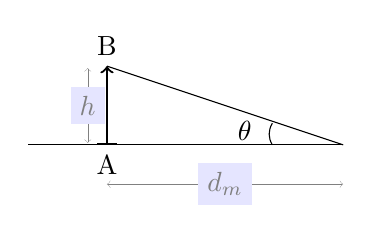
\begin{tikzpicture}[scale=1] % from physagreg
                    \def \taillehaut{2};
                    \def \taillebas{2};
                    \def \xA{-1};
                    \def \yB{1};
                    \def \xAA {(\xA*\f)/(\xA+\f)};
                    \def \yBB {(\xAA*\yB)/(\xA)};
                    \coordinate (O1) at (0,0);
                    \coordinate (A) at (\xA,0);
                    \coordinate (B) at (\xA,\yB);
                    \def \f{2};
                    \coordinate (F') at (\f,0);
                    \coordinate (A') at ({\xAA},0);
                    \coordinate (B') at ({\xAA},{\yBB});
                    \draw[|->, thick]  (A)node[below]{A}--(B)node[above]{B};
                    % Grandeurs
                    \node[left=.22cm, inner sep=0] (Aa) at (A) {};
                    \node[left=.22cm, inner sep=0] (Bb) at (B) {};
                    \draw[<->, ultra thin, gray] (Aa) --
                        node[midway, fill=blue!10]{$h$} (Bb);

                    \draw[thin](-2,0)--++(4,0);
                    
                    \draw[ultra thin,gray,<->](-1,-0.5)--(2,-0.5)
                        node[midway, fill=blue!10] {$d_m$};
                    \draw (B) -- (2,0);
                    \draw (1.1,0) to [bend left] (1.1,0.275) ;
                    \node at (0.75,0.175) [] {$\theta$};
                    \oeil[shift={(2.8,0)},rotate=180];
                \end{tikzpicture}
            \end{center}
            \begin{itemize}
                \item $\t'$ l'angle sous lequel est vue l'\underline{image}
                    \underline{\underline{après le système}}, et dans le
                    grossissement \textbf{commercial} on la considère comme
                    formée à l'infini.
            \end{itemize}
            \begin{center}
                \begin{tikzpicture}[scale=1] 
                \def \taillehaut{2};
                \def \taillebas{2};
                \def \xA{-2};
                \def \yB{1};
                \coordinate (O1) at (0,0);
                \coordinate (A) at (\xA,0);
                \coordinate (B) at (\xA,\yB);
                \def \f{2};
                \coordinate (F') at (\f,0);
                
                \draw[thin](-4,0)--++(7,0);
                \draw[|->, thick] (A)node[below left]{A}--(B)
                    node[above]{B};
                % Grandeurs
                \node[left=.22cm, inner sep=0] (Aa) at (A) {};
                \node[left=.22cm, inner sep=0] (Bb) at (B) {};
                \draw[<->, ultra thin, gray] (Aa) --
                    node[midway, fill=blue!10]{$h$} (Bb);

                \draw[shift={(O1)},thick,<->,>=latex]
                    (0,-\taillebas)--(0,\taillehaut)
                    node[above]{$\mathcal{L}$};
                \draw[red,simple] (B)--(0,\yB);
                \draw[red,simple] (0,\yB)--(F');
                \draw[red, dashed] (0,\yB)--(B');
                \draw[green, simplegros] (B)--(O1)--++
                    ($1*(O1)-1*(B)$);
                \draw[green, dashed] (B)--++
                    ($1*(B)-1*(O1)$);
                
                \draw (1.2,0) to [bend left] (1.2,0.4) ;
                \node at (0.75,0.2) [] {$\theta'$};
                 
                \draw (-0.8,0) to [bend left] (-0.8,0.4) ;
                \node at (-1.25,0.2) [] {$\theta'$};
                
                \draw [->,-latex] (-2.75,2) --++ (-0.5,0.30);
                \node at (-2.5,2.2)  {\tiny Image};
                 
                \draw[ultra thin,gray,<->](-2,-0.5)--(-0.05,-0.5)
                    node[midway,fill=blue!10] {$\text{f'}$};
                 
                \oeil[shift={(2.8,0)},rotate=180];
                \end{tikzpicture}
            \end{center}
            Dans le cas présent l'image n'est pas formée à l'infini, et on
            n'indique pas la distance de l'œil à l'objet : on va donc définir le
            grossissement commercial de la loupe. Avec $h$ la taille de l'objet,
            les schémas précédents donnent
            \[ \boxed{G = \frac{\t'}{\t}
                        = \frac{\frac{h}{f'}}{\frac{h}{d_m}}
                        = \frac{d_m}{f'}} \]
   \end{enumerate} 
\end{NCdemo}

\begin{NCexem}[breakable]{Résultats}
    \begin{enumerate}
        \item $\boxed{\OAp = \SI{-4}{cm}}$ ;
        \item On a :
    \end{enumerate}
        \begin{center}
            \begin{tikzpicture}[]
                % Axe optique
                \draw[thin, ->](-5,0)--(5,0)node[below]{A.O.};
                % Lentille 
                \coordinate (O) at (0,0);
                \def \fa{4}
                \def \lsiz{2.5}
                \coordinate (F) at ($(O)+(-\fa,0)$);
                \coordinate (Fp) at ($(O)+(\fa,0)$);
        
                \foreach \x/\z in {O/\fa}{
                    \draw[shift={(\x)}] (0,0)
                        node[below right] {O$_{}$};
                    \draw[shift={(\x)}] (\z,2pt) --++ (0,-4pt)
                        node[below right] {F$'_{}$};
                    \draw[shift={(\x)}] ({-\z},2pt) --++ (0,-4pt)
                        node[below left] {F$_{}$};
                }
        
                \draw[shift={(O)}, thick,
                    <->, >=latex, name path=L] (0,-\lsiz)--(0,\lsiz)
                    node[above]{$\Lc_{}$};
                % Objet
                \def \pos{-2}
                \def \siz{1}
                \coordinate (A) at ($(O)+(\pos,0)$);
                \coordinate (B) at ($(A)+(0,\siz)$);
                \draw[->, Purple!70] (A) 
                    node[below] {A}
                    -- (B)
                    node[above] {B};
                % Rayons pour objet entre le foyer et
                %le centre d'une lentille convergente
                % Lengths
                \len{(A)}{(O)}{\posi}
                \len{(A)}{(B)}{\size}
                \len{(O)}{(F)}{\foc}
                % Rayon 1
                \draw[brandeisblue, simple] (B) -- (O);
                \draw[orange!70, simple] (O) --++ ($(O)-(B)$);
                \def \mut{1.2}
                \draw[orange!70, simplerev,
                    dashed, name path=OBp] (B) --++ ($\mut*(B)-\mut*(O)$);
                % Rayon 2
                \draw[brandeisblue, double] (B) --++ (\posi,0) coordinate (I);
                \def \mut{1.2}
                \draw[orange!70, double] (I) --++ ($\mut*(Fp)-\mut*(I)$);
                \draw[orange!70, doublerev,
                    dashed, name path=IBp] (I) --++ ($-\mut*(Fp)+\mut*(I)$);
                % Rayon 3
                \def \intsiz{\size*\foc/(\posi-\foc)}
                \draw[brandeisblue, triple] (B) -- (F)
                --++ (\foc,-{\intsiz}) coordinate (E);
                \def \mut{1.2}
                \draw[orange!70, triple] (E) --++ (\mut*\foc,0);
                \draw[orange!70, triplerev,
                dashed, name path=EBp] (E) --++ (-\mut*\foc,0);
                % Image
                \path[name intersections={of=OBp and IBp, by=B\bp}];
                \coordinate (A\bp) at ($(B\bp)+(0,{\intsiz})$);
                \draw[->, Red!70] (A\bp) 
                node[below] {A\bp}
                -- (B\bp)
                node[above] {B\bp};
                % Grandeurs
                \node[below] (O) at (O) {};
                \node[below] (Fp) at (Fp) {};
                \draw[<->, ForestGreen] (O) --
                    node[below, midway]{\scriptsize $\OF = \SI{4}{cm}$} (Fp);
                \node[below] (A) at (A) {};
                \draw[<->, ForestGreen] (A) --
                    node[below, midway]{\scriptsize $\OA = \SI{-2}{cm}$} (O);
                \node[left] (A) at (A) {};
                \node[left] (B) at (B) {};
                \draw[<->, ForestGreen] (A) --
                node[above, midway, sloped]
                {\fontsize{6}{6}{$\AB = \SI{1}{cm}$}} (B);
                \node[left] (Ap) at (A\bp) {};
                \node[left] (Bp) at (B\bp) {};
                \draw[<->, ForestGreen] (Ap) --
                node[above, midway, sloped]
                {\fontsize{6}{6}{$\ABp = \SI{2}{cm}$}} (Bp);
                \node[below=.5cm] (O) at (0,0) {};
                \node[below=.5cm] (Ap) at (A\bp) {};
                \draw[<->, ForestGreen] (Ap) --
                    node[below, midway]{\scriptsize $\OAp = \SI{-4}{cm}$} (O);
            \end{tikzpicture}
        \end{center}
    \begin{enumerate}[resume]
        \item Image \underline{virtuelle} ;
        \item $\boxed{\ABp = \SI{2}{cm}}$ ;
        \item Application : $\boxed{G = 6.25}$
    \end{enumerate}
\end{NCexem}

\newpage

\section{Œil réduit et accomodation}
\begin{NCdefi}{Données}
    \begin{minipage}{0.5\linewidth}
        \begin{enumerate}
            \item Rétine = écran, \smallbreak
                cristallin = lentille ;
            \item Au repos, $A$ à l'infini ;
            \item Au \textit{proximum}, $A$ à \SI{25}{cm} \smallbreak
                ($\OA = \SI{-25}{cm}$).
        \end{enumerate}
    \end{minipage}
    \begin{minipage}{0.5\linewidth}
        \begin{center}
            \begin{tikzpicture}[scale=.9]
                % Axe optique
                \draw[thin, ->](-3,0)--(3,0)node[below]{A.O.};
                % Lentille 
                \coordinate (O) at (0,0);
                \def \fa{1.5}
                \def \lsiz{2}
                \coordinate (F) at ($(O)+(-\fa,0)$);
                \coordinate (Fp) at ($(O)+(\fa,0)$);

                \foreach \x/\z in {O/\fa}{
                    \draw[shift={(\x)}] (0,0)
                        node[below right] {O$_{}$};
                }

                \draw[shift={(O)}, thick,
                    <->, >=latex, name path=L] (0,-\lsiz)--(0,\lsiz)
                    node[above]{$\Lc_{}$};
                % Écran
                \def\ecsiz{4}
                \draw[dotted] ($(2.9,0)+(0,-\ecsiz/2)$)
                    --++ (0,\ecsiz);
                \node[above right] (E) at (2.9,0) {E};
                % Objet
                \def \pos{-2.9}
                \def \siz{1.5}
                \coordinate (Ar) at ($(O)+(\pos,0)$);
                \coordinate (Br) at ($(Ar)+(0,\siz)$);
                % Rayons pour objet avant foyer d'une lentille convergente
                % Lengths
                \len{(Ar)}{(O)}{\posi}
                \len{(Ar)}{(Br)}{\size}
                \len{(O)}{(F)}{\foc}
                % Rayon 2
                \draw[brandeisblue, double] (Br) --++ (\posi,0)
                    node[above, midway, brandeisblue] {Remotum} coordinate (Ir);
                % Objet
                \def \pos{-2.5}
                \def \siz{1}
                \coordinate (A) at ($(O)+(\pos,0)$);
                \coordinate (B) at ($(A)+(0,\siz)$);
                \draw[->, Purple!70] (A) 
                    node[below] {A}
                    -- (B)
                    node[left] {B};
                % Rayons pour objet avant foyer d'une lentille convergente
                % Lengths
                \len{(A)}{(O)}{\posi}
                \len{(A)}{(B)}{\size}
                \len{(O)}{(F)}{\foc}
                % Rayon 2
                \draw[brandeisblue, simple] (B) --++ (\posi,0)
                node[below, midway] {Proximum} coordinate (I);
                % Grandeurs
                \node[below] (Og) at (O) {};
                \node[below] (Ag) at (A) {};
                \draw[<->, ForestGreen] (Ag) --
                node[below, midway, sloped]{\scriptsize $\SI{-25}{cm}$} (Og);
                % Grandeurs
                \node[above=1em, inner sep=0] (Ig) at (Ir) {};
                \node[above=1em, inner sep=0] (Brg) at (Br) {};
                \draw[<->, ForestGreen, dashed] (Brg) --
                node[above, midway, sloped]{\scriptsize $-\infty$} (Ig);
                % Grandeurs
                \node[above] (Og) at (O) {};
                \node[above] (Eg) at (2.9,0) {};
                \draw[<->, ForestGreen] (Og) --
                node[above, midway, sloped]{\scriptsize $\SI{22.3}{mm}$} (Eg);
                
            \end{tikzpicture}
        \end{center}
    \end{minipage}
\end{NCdefi}

\begin{tcbraster}[raster columns=2, raster equal height=rows]
    \begin{NCprop}{Résultats attendus}
        \begin{enumerate}
            \item $\OF _\mathrm{repos}$ ?
            \item $\OF _\mathrm{accomodation}$ ?
        \end{enumerate}
    \end{NCprop}
    \begin{NCdemo}{Outils du cours}
        Relation de conjugaison pour une lentille mince, avec $\OAp =
        \obar{OE} = \SI{22.3}{mm}$ (le principe d'un écran c'est que l'image
        se forme dessus !!) et $\frac{1}{\OA} = 0$ quand $\OA =
        -\infty$
    \end{NCdemo}
\end{tcbraster}

\begin{NCexem}[breakable]{Résultats}
    \[ \boxed{\OF_\mathrm{repos} = \SI{22.3}{mm}}\]
    \begin{center}
        \begin{tikzpicture}[]
            % Axe optique
            \draw[thin, ->](-3,0)--(3,0)node[below]{A.O.};
            \node[above](eg) at (2.9,0) {=};
            % Lentille 
            \coordinate (O) at (0,0);
            \def \fa{2.9}
            \def \lsiz{1}
            \coordinate (F) at ($(O)+(-\fa,0)$);
            \coordinate (Fp) at ($(O)+(\fa,0)$);

            \foreach \x/\z in {O/\fa}{
                \draw[shift={(\x)}] (0,0)
                    node[below right] {O$_{}$};
                \draw[shift={(\x)}] (\z,2pt) --++ (0,-4pt)
                    node[above left] {F$'_{}$};
                \draw[shift={(\x)}] ({-\z},2pt) --++ (0,-4pt)
                    node[below left] {F$_{}$};
            }

            \draw[shift={(O)}, thick,
                <->, >=latex, name path=L] (0,-\lsiz)--(0,\lsiz)
                node[above]{$\Lc_{}$};
            % Écran
            \def\ecsiz{2}
            \draw[dotted] ($(2.9,0)+(0,-\ecsiz/2)$)
                --++ (0,\ecsiz);
            \node[above right] at (2.9,0) {E};
            % Objet
            \def \pos{-2.9}
            \def \siz{0.9}
            \coordinate (A) at ($(O)+(\pos,0)$);
            \coordinate (B) at ($(A)+(0,\siz)$);
            % Rayons pour objet avant foyer d'une lentille convergente
            % Lengths
            \len{(A)}{(O)}{\posi}
            \len{(A)}{(B)}{\size}
            \len{(O)}{(F)}{\foc}
            % Rayon 2
            \draw[brandeisblue, double] (B) --++ (\posi,0) coordinate (I);
            \def \mut{1.2}
            \draw[orange!70, double, name path=IBp] (I)
                --++ ($\mut*(Fp)-\mut*(I)$);
            \def \intsiz{\size*\foc/(\posi-\foc)}
            % Grandeurs
            \node[below] (Ag) at (A) {};
            \node[below] (Og) at (O) {};
            \draw[<->, ForestGreen, dashed] (Ag) --
            node[below, midway, sloped]{\scriptsize $-\infty$} (Og);
            % Grandeurs
            \node[below] (Fpg) at (Fp) {};
            \draw[<->, ForestGreen] (Og) --
            node[below, midway, sloped]{\scriptsize $\SI{22.3}{mm}$} (Fpg);
        \end{tikzpicture}
    \end{center}
    \[ \boxed{\OF_\mathrm{accomodation} = \SI{20.6}{mm}} \]
    \begin{center}
        \begin{tikzpicture}[]
            % Axe optique
            \draw[thin, ->](-3,0)--(3,0)node[below]{A.O.};
            \node[above](eg) at (2.9,0) {=};
            % Lentille 
            \coordinate (O) at (0,0);
            \def \fa{1.3}
            \def \lsiz{2}
            \coordinate (F) at ($(O)+(-\fa,0)$);
            \coordinate (Fp) at ($(O)+(\fa,0)$);

            \foreach \x/\z in {O/\fa}{
                \draw[shift={(\x)}] (0,0)
                    node[above right] {O$_{}$};
                \draw[shift={(\x)}] (\z,2pt) --++ (0,-4pt)
                    node[below right] {F$'_{}$};
                \draw[shift={(\x)}] ({-\z},2pt) --++ (0,-4pt)
                    node[above right] {F$_{}$};
            }

            \draw[shift={(O)}, thick,
                <->, >=latex, name path=L] (0,-\lsiz)--(0,\lsiz)
                node[above]{$\Lc_{}$};
            % Node E
            \node[above right] at (2.9,0) {E};
            % Objet
            \def \pos{-2.5}
            \def \siz{1}
            \coordinate (A) at ($(O)+(\pos,0)$);
            \coordinate (B) at ($(A)+(0,\siz)$);
            \draw[->, Purple!70] (A) 
                node[below] {A}
                -- (B)
                node[above left] {B};
            % Rayons pour objet avant foyer d'une lentille convergente
            % Lengths
            \len{(A)}{(O)}{\posi}
            \len{(A)}{(B)}{\size}
            \len{(O)}{(F)}{\foc}
            % Rayon 1
            \draw[brandeisblue, simple] (B) -- (O);
            \def\mut{1.5}
            \draw[orange!70, simple, name path=OBp] (O)
                --++ ($\mut*(O)-\mut*(B)$);
            % Rayon 2
            \draw[brandeisblue, double] (B) --++ (\posi,0) coordinate (I);
            \def \mut{2.3}
            \draw[orange!70, double, name path=IBp] (I)
            --++ ($\mut*(Fp)-\mut*(I)$);
            \def \intsiz{\size*\foc/(\posi-\foc)}
            % Rayon 3
            \draw[brandeisblue, triple] (B) -- (F)
            --++ (\foc,-{\intsiz}) coordinate (E);
            \def \mut{2.3}
            \draw[orange!70, triple, name path=EBp] (E) --++ (\mut*\foc,0);
            % Image
            \path[name intersections={of=OBp and IBp, by=B\bp}];
            \coordinate (A\bp) at ($(B\bp)+(0,{\intsiz})$);
            \draw[->, Red!70] (A\bp) 
            node[above] {A\bp}
            -- (B\bp)
            node[below right] {B\bp};
            % Grandeurs
            \node[below] (Ag) at (A) {};
            \node[below] (Og) at (O) {};
            \draw[<->, ForestGreen] (Ag) --
            node[below, midway, sloped]{\scriptsize $\SI{-25}{cm}$} (Og);
            % Grandeurs
            \node[below] (Fpg) at (Fp) {};
            \draw[<->, ForestGreen] (Og) --
            node[below, midway, sloped]{\scriptsize $\SI{20.6}{mm}$} (Fpg);
            % Grandeurs
            \node[above] (Og) at (O) {};
            \node[above] (Eg) at (2.9,0) {};
            \draw[<->, ForestGreen] (Og) --
            node[above, midway, sloped]{\scriptsize $\SI{22.3}{mm}$} (Eg);
            % Écran
            \def\ecsiz{4}
            \draw[dotted] ($(A\bp)+(0,-\ecsiz/2)$)
                --++ (0,\ecsiz);
        \end{tikzpicture}
    \end{center}

\end{NCexem}

\begin{center}
    \Huge Exercices d'entraînement
\end{center}

\section{Construction géométrique d'objets}
\subsection{}
\begin{wrapfigure}[7]{R}{0.45\linewidth}
    \vspace*{-30pt}
    \centering
    \begin{tikzpicture}[]
        % Axe optique
        \draw[thin, ->](-3,0)--(3,0)node[below]{A.O.};
        % Lentille 
        \coordinate (O) at (0,0);
        \def \fa{2.7}
        \def \lsiz{2}
        \coordinate (F) at ($(O)+(-\fa,0)$);
        \coordinate (Fp) at ($(O)+(\fa,0)$);

        \foreach \x/\z in {O/\fa}{
            \draw[shift={(\x)}] (0,0)
                node[below right] {O$_{}$};
            \draw[shift={(\x)}] (\z,2pt) --++ (0,-4pt)
                node[above right] {F$'_{}$};
            \draw[shift={(\x)}] ({-\z},2pt) --++ (0,-4pt)
                node[below left] {F$_{}$};
        }

        \draw[shift={(O)}, thick,
            <->, >=latex, name path=L] (0,-\lsiz)--(0,\lsiz)
            node[above]{$\Lc_{}$};
        % Objet
        \def \pos{2.5}
        \def \siz{1}
        \coordinate (A) at ($(O)+(\pos,0)$);
        \coordinate (B) at ($(A)+(0,\siz)$);
        \draw[->, Purple!70] (A) 
            node[below] {A}
            -- (B)
            node[above left] {B};
        % Rayons pour objet virtuel d'une lentille convergente
        % Lengths
        \len{(A)}{(O)}{\posi}
        \len{(A)}{(B)}{\size}
        \len{(O)}{(F)}{\foc}
        % Rayon 1
        \draw[brandeisblue, simple] ($2*(O)-(B)$) -- (O);
        \def \mut{1.3}
        \draw[orange!70, simple, name path=OBp] (O) --++ ($\mut*(B)-\mut*(O)$);
        % Rayon 2
        \def \mut{1.5}
        \draw[brandeisblue, double] ($(B)-(\mut*\posi,0)$)
            --++ (\mut*\posi-\posi,0) coordinate (I);
        \draw[brandeisblue, dashed, double] (I) --++ (1.2*\posi,0);
        \def \mut{1}
        \draw[orange!70, double, name path=IBp] (I) --++ ($\mut*(Fp)-\mut*(I)$);
        % Rayon 3
        \def \intsiz{\size*\foc/(\posi+\foc)}
        \draw[brandeisblue, triple] (F) --++ (\foc,{\intsiz}) coordinate (E);
        \def \mut{0.3}
        \draw[brandeisblue, dashed, triple] (E) -- (B) --++ ($\mut*(B)-\mut*(E)$);
        \draw[orange!70, triple, name path=EBp] (E) --++ (1.2*\posi,0);
        % Image
        \path[name intersections={of=OBp and IBp, by=B\bp}];
        \coordinate (A\bp) at ($(B\bp)+(0,-{\intsiz})$);
        \draw[->, Red!70] (A\bp) 
        node[below] {A\bp}
        -- (B\bp)
        node[below, right] {B\bp};
    \end{tikzpicture}
    \label{fig:consA}
\end{wrapfigure}

On a une image réelle. Pour trouver $B$, on dessine dans l'espace image les
rayons \underline{émergents} particuliers des règles de construction
\ref{rconst} et qui se croisent en $B'$ (c'est bien la finalité d'un objet qui
donne une image). On trace, depuis la lentille :

\begin{enumerate}
    \item le rayon \underline{émergent} qui passe par $O$ et par $B'$ ;
    \item le rayon \underline{émergent} qui passe par $F'$ et par $B'$ ;
    \item le rayon \underline{émergent} parallèle à l'axe optique et passant par
        $B'$.
\end{enumerate}

Le premier doit provenir d'un rayon incident passant par $B$ et par $F$. Le
second doit provenir d'un rayon incident passant par $B$ et parallèle à l'A.O.
Le dernier n'est pas dévié. \bigbreak

\subsection{}
\begin{wrapfigure}[2]{R}{0.45\linewidth}
    \vspace*{-45pt}
    \centering
    \begin{tikzpicture}[scale=1]
        % Axe optique
        \draw[thin, ->](-3,0)--(3,0)node[above]{A.O.};
        % Lentille 
        \coordinate (O) at (0,0);
        \def \fa{-2.7}
        \def \lsiz{1.5}
        \coordinate (F) at ($(O)+(-\fa,0)$);
        \coordinate (Fp) at ($(O)+(\fa,0)$);

        \foreach \x/\z in {O/\fa}{
            \draw[shift={(\x)}] (0,0)
                node[below right] {O$_{}$};
            \draw[shift={(\x)}] (\z,2pt) --++ (0,-4pt)
                node[below left] {F$'_{}$};
            \draw[shift={(\x)}] ({-\z},2pt) --++ (0,-4pt)
                node[below right] {F$_{}$};
        }

        \draw[shift={(O)}, thick,
            >-<, >=latex, name path=L] (0,-\lsiz)--(0,\lsiz)
            node[above]{$\Lc_{}$};
        % Objet
        \def \pos{0.9}
        \def \siz{0.7}
        \coordinate (A) at ($(O)+(\pos,0)$);
        \coordinate (B) at ($(A)+(0,\siz)$);
        \draw[->, Purple!70] (A) 
            node[below] {A}
            -- (B)
            node[above left] {B};
        % Rayons pour objet virtuel entre O et F d'une lentille divergente
        % Lengths
        \len{(A)}{(O)}{\posi}
        \len{(A)}{(B)}{\size}
        \len{(O)}{(F)}{\foc}
        % Rayon 1
        \draw[brandeisblue, simple] ($2*(O)-(B)$) -- (O);
        \def \mut{1.8}
        \draw[orange!70, simple, name path=OBp] (O) --++ ($\mut*(B)-\mut*(O)$);
        % Rayon 2
        \def \mut{3}
        \draw[brandeisblue, double] ($(B)-(\mut*\posi,0)$)
            --++ (\mut*\posi-\posi,0) coordinate (I);
        \draw[brandeisblue, dashed, double] (I) --++ (2*\posi,0);
        \def \mut{1.2}
        \draw[orange!70, doublerev, dashed] (I)
            --++ ($\mut*(Fp)-\mut*(I)$);
        \draw[orange!70, double, name path=IBp] (I)
            --++ ($-\mut*(Fp)+\mut*(I)$);
        % Rayon 3
            \path[name path=tripleB] (F) --++ ($3*(B)-3*(F)$);
            \path[name intersections={of=L and tripleB, by=E}];
            \def \mut{1.2}
            \draw[brandeisblue, triplerev] (E) --++ ($\mut*(B)-\mut*(F)$);
            \draw[brandeisblue, dashed, triple] (E) --++ ($\mut*(F)-\mut*(E)$);
            \draw[orange!70, triple, name path=EBp] (E) --++ (\mut*\foc,0);
            % Image
            \path[name intersections={of=OBp and IBp, by=B\bp}];
            \len{(O)}{(E)}{\intsiz}
            \coordinate (A\bp) at ($(B\bp)+(0,-{\intsiz})$);
            \draw[->, Red!70] (A\bp) 
            node[below] {A\bp}
            -- (B\bp)
            node[below, right] {B\bp};
    \end{tikzpicture}
    \label{fig:consB}
\end{wrapfigure}
\vspace*{20pt}
Même exercice, mais on échange $F$ et $F'$.
\vspace*{20pt}

\subsection{}

\begin{wrapfigure}[6]{R}{0.45\linewidth}
    \centering
    \begin{tikzpicture}[]
        % Axe optique
        \draw[thin, ->](-3,0)--(3,0)node[below]{A.O.};
        % Lentille 
        \coordinate (O) at (0,0);
        \def \fa{1.3}
        \def \lsiz{2}
        \coordinate (F) at ($(O)+(-\fa,0)$);
        \coordinate (Fp) at ($(O)+(\fa,0)$);

        \foreach \x/\z in {O/\fa}{
            \draw[shift={(\x)}] (0,0)
                node[below right] {O$_{}$};
            \draw[shift={(\x)}] (\z,2pt) --++ (0,-4pt)
                node[below right] {F$'_{}$};
            \draw[shift={(\x)}] ({-\z},2pt) --++ (0,-4pt)
                node[below left] {F$_{}$};
        }

        \draw[shift={(O)}, thick,
            <->, >=latex, name path=L] (0,-\lsiz)--(0,\lsiz)
            node[above]{$\Lc_{}$};
        % Objet
        \def \pos{-0.7}
        \def \siz{0.5}
        \coordinate (A) at ($(O)+(\pos,0)$);
        \coordinate (B) at ($(A)+(0,\siz)$);
        \draw[->, Purple!70] (A) 
            node[below] {A}
            -- (B)
            node[above left] {B};
        % Rayons pour objet entre le foyer et le centre d'une lentille convergente
        % Lengths
        \len{(A)}{(O)}{\posi}
        \len{(A)}{(B)}{\size}
        \len{(O)}{(F)}{\foc}
        % Rayon 1
        \draw[brandeisblue, simple] (B) -- (O);
        \draw[orange!70, simple] (O) --++ ($(O)-(B)$);
        \def \mut{2}
        \draw[orange!70, simplerev,
            dashed, name path=OBp] (B) --++ ($\mut*(B)-\mut*(O)$);
        % Rayon 2
        \draw[brandeisblue, double] (B) --++ (\posi,0) coordinate (I);
        \def \mut{2}
        \draw[orange!70, double] (I) --++ ($\mut*(Fp)-\mut*(I)$);
        \draw[orange!70, doublerev,
            dashed, name path=IBp] (I) --++ ($-\mut*(Fp)+\mut*(I)$);
        % Rayon 3
        \def \intsiz{\size*\foc/(\posi-\foc)}
        \draw[brandeisblue, triple] (B) -- (F)
        --++ (\foc,-{\intsiz}) coordinate (E);
        \def \mut{2}
        \draw[orange!70, triple] (E) --++ (\mut*\foc,0);
        \draw[orange!70, triplerev,
        dashed, name path=EBp] (E) --++ (-\mut*\foc,0);
        % Image
        \path[name intersections={of=OBp and IBp, by=B\bp}];
        \coordinate (A\bp) at ($(B\bp)+(0,{\intsiz})$);
        \draw[->, Red!70] (A\bp) 
        node[left] {A\bp}
        -- (B\bp)
        node[above] {B\bp};
    \end{tikzpicture}
    \label{fig:consC}
\end{wrapfigure}

On a une image virtuelle. On doit tracer dans l'espace image trois rayons
d'intérêt dont la \underline{prolongation dans le sens} \underline{opposé à
celle de la marche des rayons} passe par $B'$. Même principe ensuite.

\begin{enumerate}
    \item le rayon qui passe par $O$ et par $B'$ ;
    \item le rayon qui passe par $F'$ et par $B'$ ;
    \item et le rayon parallèle à l'axe optique et passant par $B'$.
\end{enumerate} \bigbreak

Le premier doit provenir d'un rayon incident passant par $B$ et par $F$. Le
second doit provenir d'un rayon incident passant par $B$ et parallèle à l'A.O.
Le dernier n'est pas dévié.

\subsection{}
\begin{wrapfigure}[4]{R}{0.45\linewidth}
    \vspace*{-60pt}
    \centering
    \begin{tikzpicture}[]
        % Axe optique
        \draw[thin, ->](-3,0)--(3,0)node[below]{A.O.};
        % Lentille 
        \coordinate (O) at (0,0);
        \def \fa{-0.75}
        \def \lsiz{1.5}
        \coordinate (F) at ($(O)+(-\fa,0)$);
        \coordinate (Fp) at ($(O)+(\fa,0)$);

        \foreach \x/\z in {O/\fa}{
            \draw[shift={(\x)}] (0,0)
                node[below right] {O$_{}$};
            \draw[shift={(\x)}] (\z,2pt) --++ (0,-4pt)
                node[below left] {F$'_{}$};
            \draw[shift={(\x)}] ({-\z},2pt) --++ (0,-4pt)
                node[below right] {F$_{}$};
        }

        \draw[shift={(O)}, thick,
            >-<, >=latex, name path=L] (0,-\lsiz)--(0,\lsiz)
            node[above]{$\Lc_{}$};
        % Objet
        \def \pos{1.5}
        \def \siz{-0.5}
        \coordinate (A) at ($(O)+(\pos,0)$);
        \coordinate (B) at ($(A)+(0,\siz)$);
        \draw[->, Purple!70] (A) 
            node[above] {A}
            -- (B)
            node[below] {B};
        % Rayons pour objet virtuel après F d'une lentille divergente
        % Lengths
        \len{(A)}{(O)}{\posi}
        \len{(A)}{(B)}{\size}
        \len{(O)}{(F)}{\foc}
        % Rayon 1
        \draw[brandeisblue, simple, name path=OBp] ($2*(O)-1.2*(B)$) -- (O);
        \def \mut{1.8}
        \draw[orange!70, simple] (O) --++ ($\mut*(B)-\mut*(O)$);
        % Rayon 2
        \def \mut{2.2}
        \draw[brandeisblue, double] ($(B)-(\mut*\posi,0)$)
            --++ (\mut*\posi-\posi,0) coordinate (I);
        \draw[brandeisblue, dashed, double] (I) --++ (2*\posi,0);
        \def \mut{2.2}
        \draw[orange!70, doublerev, dashed, name path=IBp] (I)
            --++ ($\mut*(Fp)-\mut*(I)$);
        \def \mut{1.2}
        \draw[orange!70, double] (I)
            --++ ($-\mut*(Fp)+\mut*(I)$);
        % Rayon 3
        \path[name path=tripleB] (B) --++ ($3*(F)-3*(B)$);
        \path[name intersections={of=L and tripleB, by=E}];
        \def \mut{1.5}
        \draw[brandeisblue, triplerev] (E) --++ ($\mut*(F)-\mut*(B)$);
        \def \mut{2.2}
        \draw[brandeisblue, dashed, triple] (E) --++ ($\mut*(F)-\mut*(E)$);
        \draw[orange!70, triple] (E) --++ (\mut*\foc,0);
        \draw[orange!70, triplerev,
        dashed, name path=EBp] (E) --++ (-\mut*\foc,0);
        % Image
        \path[name intersections={of=OBp and IBp, by=B\bp}];
        \len{(O)}{(E)}{\intsiz}
        \coordinate (A\bp) at ($(B\bp)-(0,{\intsiz})$);
        \draw[->, Red!70] (A\bp) 
        node[below] {A\bp}
        -- (B\bp)
        node[above] {B\bp};
    \end{tikzpicture}
    \label{fig:consD}
\end{wrapfigure}
\vspace*{20pt}
Même exercice, mais on échange $F$ et $F'$.
\vspace*{20pt}

\section{Trouver la lentille}
Pour cet exercice, il faut étudier les liens entre objet et image avec le centre
$O$ et le foyer image d'une lentille. On se rend alors compte qu'en traçant une
droite de $B$ à $B'$, il est naturel de trouver $O$ à l'intersection de cette
droite et de l'axe optique. On peut faire ça pour chaque schéma, et il ne reste
qu'à trouver le foyer image.

Pour cela, après avoir trouvé $O$ et tracé une lentille (pour le moment, ni
convergente ni divergente), il suffit de tracer un rayon partant de $B$ et
parallèle à l'axe optique qui, une fois arrivé à la lentille, doit continuer
jusqu'à passer en $B'$. L'intersection de ce rayon et de l'axe optique donne
l'emplacement de $F'$. Il faut cependant faire attention à bien savoir si ce
sont les prolongations des rayons ou les rayons eux-mêmes qui partent de $B$ ou
qui arrivent en $B'$. Les schémas sont en ligne sur Claroline.

\section{Relation de conjugaison}

Dans cet exercice, on veut démontrer la relation de conjugaison du cours
\begin{equation*}
	\boxed{\dfrac{1}{\overline{OF^\prime}} =
    \dfrac{1}{\overline{OA^\prime}} - \dfrac{1}{\overline{OA}}}
\end{equation*}
en se servant uniquement des rayons particuliers que l'on peut construire pour
toute lentille mince, à savoir celui qui passe par le centre optique et ceux qui
passent par les foyers. Dans ce genre de démonstration, il est très important de
faire attention à l'utilisation des valeurs algébriques des longueurs lorsqu'on
applique les formules de trigonométrie. Une bonne technique consiste à utiliser
des angles inférieurs à $90\degres$ pour lesquels toutes les fonctions
trigonométriques sont positives, et à utiliser alors des grandeurs algébriques
positives dans l'écriture de ces formules.

\begin{center}
    \begin{tikzpicture}[]
        % Axe optique
        \draw[thin, ->](-3,0)--(3,0)node[below]{A.O.};
        % Lentille 
        \coordinate (O) at (0,0);
        \def \fa{1.5}
        \def \lsiz{2}
        \coordinate (F) at ($(O)+(-\fa,0)$);
        \coordinate (Fp) at ($(O)+(\fa,0)$);

        \foreach \x/\z in {O/\fa}{
            \draw[shift={(\x)}] (0,0)
                node[below right] {O$_{}$};
            \draw[shift={(\x)}] (\z,2pt) --++ (0,-4pt)
                node[above] {F$'_{}$};
            \draw[shift={(\x)}] ({-\z},2pt) --++ (0,-4pt)
                node[below left] {F$_{}$};
        }

        \draw[shift={(O)}, thick,
            <->, >=latex, name path=L] (0,-\lsiz)--(0,\lsiz)
            node[above]{$\Lc_{}$};
        % Objet
        \def \pos{-3}
        \def \siz{1}
        \coordinate (A) at ($(O)+(\pos,0)$);
        \coordinate (B) at ($(A)+(0,\siz)$);
        \draw[->, Purple!70] (A) 
            node[below] {A}
            -- (B)
            node[above left] {B};
        % Rayons pour objet avant foyer d'une lentille convergente
        % Lengths
        \len{(A)}{(O)}{\posi}
        \len{(A)}{(B)}{\size}
        \len{(O)}{(F)}{\foc}
        % Rayon 1
        \draw[brandeisblue, simple, name path=B] (B) -- (O);
        \def\mut{1.2}
        \draw[orange!70, simple, name path=OBp] (O)
            --++ ($\mut*(O)-\mut*(B)$);
        % Rayon 2
        \draw[brandeisblue, double] (B) --++ (\posi,0) coordinate (I);
        \def \mut{2}
        \draw[orange!70, double, name path=IBp] (I)
            --++ ($\mut*(Fp)-\mut*(I)$);
        \node[above right] (Bpp) at (I) {B\bp\bp};
        \def \intsiz{\size*\foc/(\posi-\foc)}
        % Image
        \path[name intersections={of=OBp and IBp, by=B\bp}];
        \coordinate (A\bp) at ($(B\bp)+(0,{\intsiz})$);
        \draw[->, Red!70] (A\bp) 
        node[above] {A\bp}
        -- (B\bp)
        node[below right] {B\bp};
        % Intersection avec verticale
        \def\vertsiz{5}
        \path[name path=V] (-.75,-\vertsiz/2)
            --++ (0,\vertsiz);
        % Define intersection
        \path[name intersections={of=B and V, by=BV}];
        % Angle
        \draw[ForestGreen] (-.75,0) to [bend left] node[midway, left]{$\a$} (BV);
        % Intersection avec verticale
        \def\vertsiz{5}
        \path[name path=Vb] (.75,-\vertsiz/2)
        --++ (0,\vertsiz);
        % Define intersection
        \path[name intersections={of=OBp and Vb, by=OV}];
        % Angle
        \draw[ForestGreen] (.75,0) to[bend left] node[midway, right]{$\a$} (OV);
        % Intersection avec verticale
        \def\vertsiz{5}
        \path[name path=Vdb] (.85,-\vertsiz/2)
        --++ (0,\vertsiz);
        % Define intersection
        \path[name intersections={of=IBp and Vdb, by=beta}];
        % Angle
        \draw[ForestGreen] (.85,0) to[bend left] node[midway, left]{$\b$} (beta);
        % Intersection avec verticale
        \def\vertsiz{5}
        \path[name path=Vdbb] (2.15,-\vertsiz/2)
        --++ (0,\vertsiz);
        % Define intersection
        \path[name intersections={of=Vdbb and IBp, by=betab}];
        % Angle
        \draw[ForestGreen] (2.15, 0) to[bend left] node[midway, right]{$\b$} (betab);
    \end{tikzpicture}
\end{center}
Pour trouver la relation de conjugaison, nous utilisons le triangle $ABO$ dans
lequel l'angle $\alpha \equiv \widehat{AOB}$ permet d'obtenir la relation

\begin{equation*}
	\tan(\alpha) = \dfrac{\overline{AB}}{\overline{AO}}
\end{equation*}
Dans le triangle $OA^\prime B^\prime$, l'angle de même valeur $\widehat{A^\prime
O B^\prime} = \alpha$ permet d'obtenir
\begin{equation*}
	\tan(\alpha) = \dfrac{\overline{B^\prime A^\prime}}{\overline{OA^\prime}}
\end{equation*}
On démontre ainsi immédiatement la formule du grandissement
\begin{equation*}
	\dfrac{\overline{AB}}{\overline{AO}} =
    \dfrac{\overline{B^\prime A^\prime}}{\overline{OA^\prime}}
    \iff
    \boxed{\dfrac{\overline{A^\prime B^\prime}}{\overline{AB}}
    = \dfrac{\overline{OA^\prime}}{\overline{OA}}}
\end{equation*}
Nous définissons ensuite le point intermédiaire $B^{\prime\prime}$ qui est
l'intersection du rayon partant de $B$ parallèlement à l'axe optique et de la
lentille. Ainsi, dans le triangle $OB^{\prime\prime}F^\prime$, l'angle
$\beta\equiv \widehat{F^\prime O B^{\prime\prime}}$ donne
\begin{equation*}
	\tan(\beta) = \dfrac{\overline{OB^{\prime\prime}}}{\overline{OF^\prime}}
    = \dfrac{\overline{AB}}{\overline{OF^\prime}}
\end{equation*}
Dans l'autre triangle $F^\prime A^\prime B^\prime$, l'angle de même valeur
$\widehat{B^\prime F^\prime A^\prime} = \beta$ donne
\begin{equation*}
	\tan(\beta) =
    \dfrac{\overline{B^\prime A^\prime}}{\overline{F^\prime A^\prime}}
\end{equation*}
On a donc
\begin{equation*}
	\dfrac{\overline{AB}}{\overline{OF^\prime}} =
    \dfrac{\overline{B^\prime A^\prime}}{\overline{F^\prime A^\prime}}
    \iff
    \dfrac{\overline{A^\prime B^\prime}}{\overline{AB}}
    = \dfrac{\overline{A^\prime F^\prime}}{\overline{OF^\prime}}
\end{equation*}
En remplaçant dans la formule de grandissement, et en utilisant la décomposition
\begin{equation*}
	\overline{A^\prime F^\prime} = \overline{A^\prime O} + \overline{OF^\prime}
    = -\overline{OA^\prime} + \overline{OF^\prime}
\end{equation*}
on a donc en divisant les deux côtés par $\overline{OA^\prime}$
\begin{equation*}
	\dfrac{\overline{OA^\prime}}{\overline{OA}} =
    \dfrac{\overline{A^\prime F^\prime}}{\overline{OF^\prime}} =
    - \dfrac{\overline{OA^\prime}}{\overline{OF^\prime}} + 1
    \iff
    \boxed{\dfrac{1}{\overline{OF^\prime}} =
    \dfrac{1}{\overline{OA^\prime}} - \dfrac{1}{\overline{OA}}}
\end{equation*}

\section{Lentilles inconnues}
Cet exercice peut paraître déroutant, mais il faut simplement s'en tenir à ce
qu'on peut faire. On sait que les rayons émergents doivent se croiser en $B'$,
par définition. On peut tracer le rayon de $B'$ à $O$, c'est toujours une source
sûre. Ce rayon doit également passer par $B$ : étant donné qu'on a la position
$A$, on en déduit la position de $B$ qui est à la verticale de $A$ et sur ce
rayon.

Ensuite, on peut tracer le rayon émergent parallèle à l'axe optique qui
passe par $B'$ (en prolongation). On sait qu'il doit partir de $B$ et coupe
l'axe optique en $F$ : on a trouvé $B$ et $F$ !

\begin{minipage}{0.45\linewidth}
    \begin{center}
        \begin{tikzpicture}[scale=0.9]
            % Axe optique
            \draw[thin, ->](-3,0)--(3,0)node[above]{A.O.};
            % Lentille 
            \coordinate (O) at (0,0);
            \def \fa{2.7}
            \def \lsiz{2}
            \coordinate (F) at ($(O)+(-\fa,0)$);
            \coordinate (Fp) at ($(O)+(\fa,0)$);

            \foreach \x/\z in {O/\fa}{
                \draw[shift={(\x)}] (0,0)
                    node[below right] {O$_{}$};
                \draw[shift={(\x)}] (\z,2pt) --++ (0,-4pt)
                    node[below right] {F$'_{}$};
                \draw[shift={(\x)}] ({-\z},2pt) --++ (0,-4pt)
                    node[below left] {F$_{}$};
            }

            \draw[shift={(O)}, thick,
                <->, >=latex, name path=L] (0,-\lsiz)--(0,\lsiz)
                node[above]{$\Lc_{}$};
            % Objet
            \def \pos{-1}
            \def \siz{0.7}
            \coordinate (A) at ($(O)+(\pos,0)$);
            \coordinate (B) at ($(A)+(0,\siz)$);
            \draw[->, Purple!70] (A) 
                node[below] {A}
                -- (B)
                node[above left] {B};
            % Rayons pour objet entre le foyer et le centre d'une lentille convergente
            % Lengths
            \len{(A)}{(O)}{\posi}
            \len{(A)}{(B)}{\size}
            \len{(O)}{(F)}{\foc}
            % Rayon 1
            \draw[brandeisblue, simple] (B) -- (O);
            \draw[orange!70, simple] (O) --++ ($(O)-(B)$);
            \def \mut{2}
            \draw[orange!70, simplerev,
                dashed, name path=OBp] (B) --++ ($\mut*(B)-\mut*(O)$);
            % Rayon 2
            \draw[brandeisblue, double] (B) --++ (\posi,0) coordinate (I);
            \def \mut{1.2}
            \draw[orange!70, double] (I) --++ ($\mut*(Fp)-\mut*(I)$);
            \draw[orange!70, doublerev,
                dashed, name path=IBp] (I) --++ ($-\mut*(Fp)+\mut*(I)$);
            % Rayon 3
            \def \intsiz{\size*\foc/(\posi-\foc)}
            \draw[brandeisblue, triple] (B) -- (F)
            --++ (\foc,-{\intsiz}) coordinate (E);
            \def \mut{1.2}
            \draw[orange!70, triple] (E) --++ (\mut*\foc,0);
            \draw[orange!70, triplerev,
            dashed, name path=EBp] (E) --++ (-\mut*\foc,0);
            % Image
            \path[name intersections={of=OBp and IBp, by=B\bp}];
            \coordinate (A\bp) at ($(B\bp)+(0,{\intsiz})$);
            \draw[->, Red!70] (A\bp) 
            node[below] {A\bp}
            -- (B\bp)
            node[below right] {B\bp};
        \end{tikzpicture}
    \end{center}
\end{minipage}
\hfill
\begin{minipage}{0.45\linewidth}
    \begin{center}
        \begin{tikzpicture}[scale=0.9]
            % Axe optique
            \draw[thin, ->](-3,0)--(3,0)node[below]{A.O.};
            % Lentille 
            \coordinate (O) at (0,0);
            \def \fa{-1}
            \def \lsiz{2}
            \coordinate (F) at ($(O)+(-\fa,0)$);
            \coordinate (Fp) at ($(O)+(\fa,0)$);

            \foreach \x/\z in {O/\fa}{
                \draw[shift={(\x)}] (0,0)
                    node[below right] {O$_{}$};
                \draw[shift={(\x)}] (\z,2pt) --++ (0,-4pt)
                    node[below left] {F$'_{}$};
                \draw[shift={(\x)}] ({-\z},2pt) --++ (0,-4pt)
                    node[below right] {F$_{}$};
            }

            \draw[shift={(O)}, thick,
                >-<, >=latex, name path=L] (0,-\lsiz)--(0,\lsiz)
                node[above]{$\Lc_{}$};
            % Objet
            \def \pos{2}
            \def \siz{-0.5}
            \coordinate (A) at ($(O)+(\pos,0)$);
            \coordinate (B) at ($(A)+(0,\siz)$);
            \draw[->, Purple!70] (A) 
                node[above] {A}
                -- (B)
                node[below] {B};
            % Rayons pour objet virtuel après F d'une lentille divergente
            % Lengths
            \len{(A)}{(O)}{\posi}
            \len{(A)}{(B)}{\size}
            \len{(O)}{(F)}{\foc}
            % Rayon 1
            \draw[brandeisblue, simple, name path=OBp] ($2*(O)-1.2*(B)$) -- (O);
            \def \mut{1.8}
            \draw[orange!70, simple] (O) --++ ($\mut*(B)-\mut*(O)$);
            % Rayon 2
            \def \mut{2.2}
            \draw[brandeisblue, double] ($(B)-(\mut*\posi,0)$)
                --++ (\mut*\posi-\posi,0) coordinate (I);
            \draw[brandeisblue, dashed, double] (I) --++ (2*\posi,0);
            \def \mut{2.2}
            \draw[orange!70, doublerev, dashed, name path=IBp] (I)
                --++ ($\mut*(Fp)-\mut*(I)$);
            \def \mut{1.2}
            \draw[orange!70, double] (I)
                --++ ($-\mut*(Fp)+\mut*(I)$);
                % Rayon 3
                \path[name path=tripleB] (B) --++ ($3*(F)-3*(B)$);
                \path[name intersections={of=L and tripleB, by=E}];
                \def \mut{1.5}
                \draw[brandeisblue, triplerev] (E) --++ ($\mut*(F)-\mut*(B)$);
                \def \mut{2.2}
                \draw[brandeisblue, dashed, triple] (E) --++ ($\mut*(F)-\mut*(E)$);
                \draw[orange!70, triple] (E) --++ (\mut*\foc,0);
                \draw[orange!70, triplerev,
                dashed, name path=EBp] (E) --++ (-\mut*\foc,0);
                % Image
                \path[name intersections={of=OBp and IBp, by=B\bp}];
                \len{(O)}{(E)}{\intsiz}
                \coordinate (A\bp) at ($(B\bp)-(0,{\intsiz})$);
                \draw[->, Red!70] (A\bp) 
                node[below] {A\bp}
                -- (B\bp)
                node[above] {B\bp};
        \end{tikzpicture}
    \end{center}
\end{minipage}

\section{Distances focales}
\begin{NCdefi}{Données}
	\begin{enumerate}
		\item $\overline{OA} = -6\,$cm ;
		\item $\overline{OA^\prime} = 2\,$cm ;
	\end{enumerate}
\end{NCdefi}

\begin{NCprop}{Résultats attendus}
	\begin{enumerate}
		\item $\OF$ ?
		\item Nature de la lentille ?
	\end{enumerate}
\end{NCprop}

\begin{NCdemo}{Outils du cours}
	\begin{enumerate}
		\item Relation de conjugaison
	\end{enumerate} 
\end{NCdemo}

\begin{NCexem}{Résultats}
	\begin{enumerate}
		\item $\boxed{\OF = 1.5\,{\rm cm}}$
        \item $\OF > 0$ donc le foyer image est à droite de la lentille, c'est
            une lentille convergente
		\item On obtient :
            \begin{center}
                \begin{tikzpicture}[scale=.5]
                    % Axe optique
                    \draw[thin, ->](-6.5,0)--(6.5,0)node[below]{A.O.};
                    % -----------------------------------------------------------
                    % Lentille 
                    \coordinate (O) at (0,0);
                    \def \fa{1.5}
                    \def \lsiz{4}
                    \coordinate (F) at ($(O)+(-\fa,0)$);
                    \coordinate (Fp) at ($(O)+(\fa,0)$);

                    \foreach \x/\z in {O/\fa}{
                        \draw[shift={(\x)}] (0,0)
                            node[below right] {O$_{}$};
                        \draw[shift={(\x)}] (\z,4pt) --++ (0,-8pt)
                            node[above left=.5pt] {F$'_{}$};
                        \draw[shift={(\x)}] ({-\z},4pt) --++ (0,-8pt)
                            node[below left] {F$_{}$};
                    }

                    \draw[shift={(O)}, thick,
                        <->, >=latex, name path=L] (0,-\lsiz)--(0,\lsiz)
                        node[above]{$\Lc_{}$};
                    % -----------------------------------------------------------
                    % Objet
                    \def \pos{-6}
                    \def \siz{2}
                    \coordinate (A) at ($(O)+(\pos,0)$);
                    \coordinate (B) at ($(A)+(0,\siz)$);
                    \draw[->, Purple!70] (A) 
                        node[below] {A}
                        -- (B)
                        node[above, left] {B};
                    % Rayons pour objet avant foyer d'une lentille convergente
                    % Lengths
                    \len{(A)}{(O)}{\posi}
                    \len{(A)}{(B)}{\size}
                    \len{(O)}{(F)}{\foc}
                    % Rayon 1
                    \draw[brandeisblue, simple] (B) -- (O);
                    \draw[orange!70, simple, name path=OBp] (O) --++ ($(O)-(B)$);
                    % Rayon 2
                    \draw[brandeisblue, double] (B) --++ (\posi,0) coordinate (I);
                    \def \mut{2}
                    \draw[orange!70, double, name path=IBp] (I)
                        --++ ($\mut*(Fp)-\mut*(I)$);
                    % Rayon 3
                    \def \intsiz{\size*\foc/(\posi-\foc)}
                    \draw[brandeisblue, triple] (B) -- (F)
                        --++ (\foc,-{\intsiz}) coordinate (E);
                    \def \mut{2}
                    \draw[orange!70, triple, name path=EBp] (E) --++ (\mut*\foc,0);
                    % Image
                    \path[name intersections={of=OBp and IBp, by=B\bp}];
                    \coordinate (A\bp) at ($(B\bp)+(0,{\intsiz})$);
                    \draw[->, Red!70] (A\bp) 
                    node[above] {A\bp}
                    -- (B\bp)
                    node[below, right] {B\bp};
                    % -----------------------------------------------------------
                \end{tikzpicture}
            \end{center}
	\end{enumerate}
\end{NCexem}

\section{Les petits angles}

L'objectif de cet exercice est de montrer quantitativement à quoi correspond
« l'approximation des petits angles » nécessaire à l'applicabilité des conditions
de Gauss. Tout d'abord, rappelons que la relation entre les valeurs d'un angle
$\alpha$ en degré et en radians est
\begin{equation}
	\alpha({\rm rad}) = \dfrac{\alpha(^{\rm o})\times 2\pi}{360}
\end{equation}
Ainsi, nous pouvons remplir le tableau
\begin{table*}[h!]
	\centering
	\begin{tabular}{|c|c|c|c|}
		\hline
		$i$ ($^{\rm o}$) & $i$ (rad) & $\sin(i)$ & Ecart relatif (\%) \\
		\hline
		8 & $0.140$ & $0.140$ & 0 \\
		\hline
		10 & $0.174$ & $0.173$ & $0.57$ \\
		\hline
		12 & $0.209$ & $0.207$ & $0.9$ \\
		\hline
		15 & $0.262$ & $0.259$ & $1.2$ \\
		\hline
		18 & $0.314$ & $0.309$ & $1.6$ \\
		\hline
		20 & $0.349$ & $0.342$ & 2 \\
		\hline
		25 & $0.436$ & $0.423$ & $3.1$ \\
		\hline
	\end{tabular}
\end{table*}
Ce tableau montre que même pour des angles de $25^{\rm o}$, l'erreur relative
entre l'angle et son sinus est de l'ordre du pourcentage, validant les
conditions de Gauss.

\theendnotes

\chapter{Miroirs et dioptres plans}
\vspace*{-47pt}
\begin{center}
    \Huge Exercices d'application
\end{center}

\section{Miroir plan et tracé des rayons}
\subsection{}
\begin{minipage}{0.75\linewidth}
    On a intersection des rayons incidents avant le miroir, c'est un objet réel.
    L'image de cet objet par le miroir est son symétrique par rapport au plan du
    miroir : elle est virtuelle. Les rayons émergents passent par cette image
    (mais sont en pointillés derrière le miroir).
\end{minipage}
\begin{minipage}[c]{0.25\linewidth}
    \begin{flushright}
        \begin{tikzpicture}[use optics]
            % Miroir
            \node[mirror, rotate=-90] (M) at (0,-1) {};
            \node[right] at (M.north) {M};
            % Objet
            \coordinate (A) at (-0.25,0);
            \node[above, color=Purple!70] at (A) {A};
            \node[color=Purple!70] at (A) {$\times$};
            % Projection
            \coordinate (H) at ($(M.north)!(A)!(M.south)$);
            \node[above right, gray!70] at (H) {H};
            \node[gray!70] at (H) {$\times$};
            \draw[dashed, gray!70] (A) -- (H) --++ ($(H)-(A)$) coordinate (Ap);
            % Image
            \node[below, Red!70] at (Ap) {A$'$};
            \node[Red!70] at (Ap) {$\times$};
            % Rayons
            \draw[brandeisblue, simple]
                (A) -- ([shift={(-0.15,0)}]M.north) coordinate (Id);
            \draw[brandeisblue, double]
                (A) -- ([shift={(0.15,0)}]M.south) coordinate (Ig);
            \draw[dashed, orange!70, simple] (Ap) -- (Id);
            \draw[dashed, orange!70, double] (Ap) -- (Ig);
            \draw[orange!70, simple] (Id) --++ ($(Id)-(Ap)$);
            \draw[orange!70, double] (Ig) --++ ($(Ig)-(Ap)$);
        \end{tikzpicture}
    \end{flushright}
\end{minipage}


\subsection{}
\begin{minipage}{0.75\linewidth}
    Les rayons incidents se croisent après le miroir. On a un objet virtuel. Son
    image par le miroir plan est son symétrique par rapport au plan du miroir.
    C'est donc une image réelle (au-dessus du miroir). Les rayons émergents
    passent par cette image.
\end{minipage}
\begin{minipage}{0.25\linewidth}
    \begin{flushright}
        \begin{tikzpicture}[use optics]
            % Miroir
            \node[mirror, rotate=-90, name path=Mpath] (M) at (0,-1) {};
            \node[right] at (M.north) {M};
            % Point
            \coordinate (A) at (0,-2);
            \node[below, Purple!70] at (A) {A};
            \node[Purple!70] at (A) {$\times$};
            % Symétrique
            \coordinate (H) at ($(M.north)!(A)!(M.south)$);
            \node[above right, gray!70] at (H) {H};
            \node[gray!70] at (H) {$\times$};
            \draw[dashed, gray!70] (A) -- (H) --++ ($(H)-(A)$) coordinate (Ap);
            \node[above, Red!70] at (Ap) {A$'$};
            \node[Red!70] at (Ap) {$\times$};
            % Rayons
            \coordinate (O1) at (-1.5,0);
            \coordinate (O2) at (-0.75,0);
            % Define intersection
            \path[name path=1A] (O1) -- (A);
            \path[name path=2A] (O2) -- (A);
            \path[name intersections={of=1A and Mpath, by=Ig}];
            \path[name intersections={of=2A and Mpath, by=Id}];
            % Draw
            \draw[brandeisblue, simple] (O1) -- (Ig);
            \draw[brandeisblue, simple, dashed] (Ig) -- (A);
            \draw[brandeisblue, double] (O2) -- (Id);
            \draw[brandeisblue, double, dashed] (Id) -- (A);
            % Émergents
            \draw[orange!70, simple] (Ig) -- (Ap);
            \draw[orange!70, double] (Id) -- (Ap);
        \end{tikzpicture}
    \end{flushright}
\end{minipage}

\subsection{}
\begin{minipage}{0.75\linewidth}
    Ici on a des rayons émergents. Leur intersection est, par définition, le
    point image. Elle se fait derrière le miroir : c'est un image virtuelle. On
    obtient l'objet associé en en faisant le symétrique par rapport au plan du
    miroir : il est donc au-dessus, et c'est un objet réel.
\end{minipage}
\begin{minipage}{0.25\linewidth}
    \begin{flushright}
        \begin{tikzpicture}[use optics]
            % Miroir
            \node[mirror, rotate=-90, name path=Mpath] (M) at (0,0) {};
            \node[right] at (M.north) {M};
            % Point
            \coordinate (Ap) at (-0.5,-0.75);
            \node[below, Red!70] at (Ap) {A$'$};
            \node[Red!70] at (Ap) {$\times$};
            % Symétrique
            \coordinate (H) at ($(M.north)!(Ap)!(M.south)$);
            \node[above left, gray!70] at (H) {H};
            \node[gray!70] at (H) {$\times$};
            \draw[dashed, gray!70] (Ap) -- (H) --++ ($(H)-(Ap)$) coordinate (A);
            \node[above, Purple!70] at (A) {A};
            \node[Purple!70] at (A) {$\times$};
            % Rayons
            \coordinate (E1) at (0,1);
            \coordinate (E2) at (0.7,0.5);
            \path[name path=Eg] (Ap) -- (E1);
            \path[name path=Ed] (Ap) -- (E2);
            % Define intersection
            \path[name intersections={of=Eg and Mpath, by=Ig}];
            \path[name intersections={of=Ed and Mpath, by=Id}];
            % Draw
            \draw[orange!70, dashed, simple] (Ap) -- (Ig);
            \draw[orange!70, dashed, double] (Ap) -- (Id);
            \draw[orange!70, simple] (Ig) --++ ($2*(Ig)-2*(Ap)$);
            \draw[orange!70, double] (Id) --++ ($(Id)-(Ap)$);
            \draw[brandeisblue, simple] (A) -- (Ig);
            \draw[brandeisblue, double] (A) -- (Id);
        \end{tikzpicture}
    \end{flushright}
\end{minipage}

\section{Une grenouille intelligente}
\begin{NCdefi}{Données}
    \begin{minipage}{0.3\linewidth}
        Pour une hauteur de grenouille fixée, il y a une taille de
        nénuphar permettant à tous les rayons partant de la grenouille de ne
        pas traverser le dioptre.
    \end{minipage}
    \begin{minipage}{0.7\linewidth}
        \begin{flushright}
            \vspace*{-1cm}
            \begin{tikzpicture}[use optics, scale=0.2]
                % Dioptre
                \def\nair{1}
                \def\neau{1.33}
                \node[screen,
                    object height=8cm, rotate=90,
                    name path=Dpath]
                    (dioptre) at (0,0) {};
                \node[right] at (dioptre.south) {dioptre};
                % Milieu n1
                \node[above left] at (dioptre.south) {$n_\mathrm{air}$};
                % Milieu n2
                \def\dh{11}
                \coordinate (D1) at ($(dioptre.north)!\dh cm!-90:(dioptre.south)$);
                \fill[brandeisblue!30]
                    (dioptre.south) -- (dioptre.north) --
                    (D1) -- (D1-|dioptre.south) -- cycle;
                \node[below left] at (dioptre.south) {$n_\mathrm{eau}$};
                % Nénuphar
                \def\rsiz{11.4}
                \def\rh{0.5}
                \node[draw, scale=0.2, anchor=west,
                    minimum width=2*\rsiz cm,
                    minimum height=2*\rh cm,
                    fill=ForestGreen!80] (nenuph) at
                    ([shift={(3em,0)}]dioptre.north) {};
                % Grenouille
                \def\gsiz{10}
                \draw[Circle-{[Purple!70]Circle}]
                    (nenuph.south) coordinate (Atop)
                    --++ (0,-\gsiz) coordinate (A);
                % Point
                \node[left, Purple!70] at (A) {A};
                \node[Purple!70] at (A) {$\times$};
                % Rayons
                \foreach \i/\n in {30/1, 50/2, 60/3, 70/4}{
                    \path[name path=AI\n] (A) --++ (\i:25cm);
                    % Define intersection
                    \path[name intersections={of=Dpath and AI\n, by=I\n}];
                    \draw[brandeisblue, dotted, simple] (A) -- (I\n);
                }
                \path[name path=AI0] (A) --++ (41.25:30cm);
                % Define intersection
                \path[name intersections={of=AI0 and Dpath, by=I0}];
                \draw[brandeisblue, simple] (A) -- (I0);
                % Snell
                \foreach \i/\n in {50/2, 60/3, 70/4}{
                    \draw[orange!70, dotted, simple] (I\n) --++
                        ({90-asin(\neau*sin(90-\i)/\nair)}:7cm);
                }
                \draw[orange!70, simple] (I0) --++ (0:15cm) coordinate (Aend);
                % Réflexion
                \draw[orange, dotted, simple, rotate=-90] (I1) --++ (60:7cm);
                % Normal
                \def\hsiz{5}
                \draw[gray!50, dashed, name path=Hpath]
                ([shift={(0,\hsiz)}]I0) coordinate (Htop) --
                ([shift={(0,-\hsiz)}]I0) coordinate (Hbot);
                % Define intersection
                \path[name intersections={of=Hpath and Dpath, by=H}];
                \node[gray!70, below right] at (H) {H};
                \node[gray!70] at (H) {$\times$};
                % Draw angles
                \pic[scale=0.2,
                angle radius=2cm, angle eccentricity=1.7,
                draw, ->, "$i_1$" alias=i1r]
                {angle=A--H--Hbot};
                \pic[scale=0.2,
                angle radius=2cm, angle eccentricity=1.7,
                draw, ->, "$i_1$" alias=i1]
                {angle=H--A--Atop};
                % Draw angles
                \pic[scale=0.2,
                angle radius=2cm, angle eccentricity=1.7,
                draw, ->,
                "\vspace{-10}\hspace{20}$i_2 = \SI{90}{\degres}$" alias=i2]
                {angle=Aend--H--Htop};
                
            \end{tikzpicture}   
        \end{flushright}
    \end{minipage}
\end{NCdefi}

\begin{NCprop}{But à atteindre}
    Origine physique de ce phénomène et traduction mathématique.
\end{NCprop}

\begin{NCdemo}{Outils du cours}
    Loi de Snell-Descartes :
    \[ n_1\sin i_1 = n_2\sin i_2\]
    et \underline{angle limite} de réfraction, tel que :
    \[ n_1\sin i_1 = n_2\sin 90\degres = n_2\]
    qui indique que pour $n_1 > n_2$, il y a un angle d'incidence à
    partir duquel il n'y a pas de rayon réfracté (les rayons réfractés font un
    angle de 90° avec la normale et sont donc parallèles au dioptre).
\end{NCdemo}

\begin{NCexem}{Conclusion}
     Pour qu'il n'y ait pas de rayon sortant de l'eau, il faut que tous les
     rayons avec un angle d'incidence plus faible que cet angle limite soient
     bloqués par le nénuphar. Un beau, grand schéma avec toutes les données
     reportées dessus mène naturellement à l'utilisation de formules
     trigonométriques de 4$^\mathrm{ème}$.
\end{NCexem}

\begin{NCcoro}{Conseil}
    Pour retenir vos formules trigonométriques, un moyen mnémotechnique :
    \begin{center}
        CAH\quad SOH \quad TOA
    \end{center}
pour \[ \cos\a = \frac{ \text{adjacent}}{ \mathrm{hypothénuse}} \quad \sin\a =
    \frac{ \text{opposé}}{ \mathrm{hypothénuse}} \quad \tan\a = \frac{
\text{opposé}}{ \mathrm{adjacent}} \]
\end{NCcoro}

\begin{NCimpo}{Important !}
    La deuxième plus \underline{grosse} erreur facile à faire mais cette fois pire que
    \textbf{tout}, c'est d'oublier que :
    \begin{center}
        \huge Les angles de la relation de Descartes sont définis entre les
        rayons et la \underline{normale} au dioptre !
    \end{center}
    Il ne faut pas prendre la surface du dioptre comme référence pour définir
    des angles.
\end{NCimpo}

\section{Le chat et le poisson}
\begin{NCdefi}{Données}
    \begin{enumerate}
        \item Aquarium $\equiv$ dioptre plan ;
        \item $n _\mathrm{eau} = 1.33$, $n _\mathrm{air} = 1$ ;
        \item $\obar{HA} = \SI{-15}{cm}$.
    \end{enumerate}
\end{NCdefi}

\begin{NCprop}{Résultats attendus}
    \begin{enumerate}
        \item Sachant que le poisson observe la lumière partant du chat (point
            $A$), que vaut $\obar{HA'}$ ?
        \item Sachant que le \underline{chat} observe la lumière partant du poisson
            (point A), que vaut $\obar{HA'}$ ?
    \end{enumerate}
\end{NCprop}

\begin{NCdemo}{Outils du cours}
    Relation de conjugaison pour un objet $A$ dans un milieu d'indice $n_1$,
    dont l'image $A'$ est dans un milieu d'indice $n_2$ :
    \[ \frac{\obar{HA'}}{\obar{HA}} = \frac{n_2}{n_1} \quad \mathrm{ou} \quad
    \frac{\obar{HA'}}{n_2} - \frac{\obar{HA}}{n_1} = 0 \]
\end{NCdemo}

\begin{NCexem}{Application}
    \begin{enumerate}
        \item Dans ce cas, $A$, le chat, est dans un milieu d'indice $n_1 = 1$ ;
            son image par le dioptre plan donne $A'$ dans le milieu d'indice
            $n_2 = n _\mathrm{eau} = 1.33$. On adapte donc la relation de conjugaison
            :
        \[ \obar{HA'} = n _\mathrm{eau}\obar{HA} = \SI{-22.5}{cm}\]
        \item Dans ce cas, $A$, le poisson, est dans un milieu d'indice $n_1 = n
            _\mathrm{eau} = 1.33$, et son image par le dioptre donne $A'$ dans l'air
            d'indice $n_2 = n _\mathrm{air} = 1$. On adapte donc la relation de
            conjugaison :
            \[ \obar{HA'} = \frac{\obar{HA}}{n _\mathrm{eau}} < \obar{HA} \]
            puisque l'on divise $\obar{HA}$ par $n _\mathrm{eau} > 1$.
    \end{enumerate}
\end{NCexem}

\begin{NCcoro}{Conseils}
    Réécrire les formules telles que vous les avez apprises en cours,
    \textbf{puis} inclure les données de l'énoncé une par une pour éviter les
    erreurs...
\end{NCcoro}

\begin{NCimpo}{Important}
    \begin{enumerate}
        \item Ne pas se tromper sur le caractère {\huge algébrique} des
            grandeurs ;
        \item Bien identifier quelle est la source, quel est l'observateur.
    \end{enumerate}
\end{NCimpo}

\begin{center}
    \Huge Exercices d'entraînement
\end{center}

\setcounter{section}{5}
\section{Lois de Snell-Descartes}
Cet exercice est d'une simplicité absolue. Et pourtant...
\begin{NCdefi}{Données}
    \begin{enumerate}
        \item Rayon incident sur un dioptre entre air et milieu d'indice $n$ :
            angle {\huge avec le dioptre} de \SI{56}{\degres} ;
        \item Différence d'angle entre rayon incident et réfléchi (« déviation
            ») de \SI{13.5}{\degres}.
    \end{enumerate}
\end{NCdefi}

\begin{NCprop}{Résultat attendu}
    Indice du liquide.
\end{NCprop}

\begin{NCdemo}{Outils du cours}
    Loi de Snell-Descartes :
    \[ n_1\sin i_1 = n_2 \sin i_2 \]
    avec $n_1$ l'indice du milieu d'indidence, $n_2$ celui du milieu de
    réfraction, $i_1$ l'angle d'incidence et $i_2$ l'angle de réfraction.
\end{NCdemo}

\begin{NCexem}{Application}
    Un bon schéma fait attentivement est \textbf{nécessaire} ici. En effet,
    les angles donnés ne sont pas ceux qu'on utilise dans la relation de
    Snell-Descartes. \bigbreak
    
    En appelant $i$ l'angle entre le rayon et le dioptre, on a
    \[ i + i_1 = 90\degres\]
    et en appelant $D$ la déviation entre les deux rayons, on a
    \[ i + 90\degres + i_2 + D = 180\degres\]

    On se débrouille pour trouver $n_2$ sachant qu'on a $i_1 = \SI{34}{\degres}$
    et $i_2 = \SI{20.5}{\degres}$. On trouve
    \[ \boxed{n_2 = 1.6} \]
\end{NCexem}

\chapter{Instruments d'optique}
\vspace*{-47pt}
\begin{center}
    \Huge Exercices d'application
\end{center}
\section{Tracés de rayons avec association de lentilles}
Les associations de lentilles ne présentent pas de difficultés particulières,
une fois les techniques de construction maîtrisées (cf. chapitre \ref{ch:O1}).

\subsection{}
Dans ce premier cas, on doit construire l'image d'un objet \underline{réel} par
l'association de deux lentilles convergentes. Il suffit pour cela de construire
l'image de l'objet initial $\ABb$ par la lentille $L_1$, image que l'on appellera
$\ABa$. C'est cette image qui servira d'objet à la lentille $L_2$, qui en
formera l'image finale $\ABp$. \bigbreak

On procède donc de la même manière que précédemment, en traçant :
\begin{enumerate}
    \item Le rayon passant par $B$ et par $O_1$ : il ne sera pas dévié ;
    \item Le rayon passant par $B$ et par $F_1$ : il émerge parallèle à
        l'\ed{A.O.}{axe optique} (optionel quand on est sûr-e de ne pas se
        tromper avec les deux autres rayons) ;
    \item Le rayon passant par $B$ et parallèle à l'A.O. : il passe par $F'_1$
        en sortie.
\end{enumerate}

On obtient un faisceau \underline{convergent} en sortie de cette lentille,
l'intersection des rayons se faisant donc dans leur prolongement dans le sens
positif. $\ABa$ est une \underline{image réelle} \underline{\underline{pour
$L_1$}}. \bigbreak

En revanche, cette image, qui est donc l'objet de la lentille $L_2$, est dans
l'espace image de celle-ci : c'est donc un \underline{objet virtuel}
\underline{\underline{pour $L_2$}}. On construit donc son image en trançant :

\begin{enumerate}
    \item Le rayon passant par $B_1$ et par $O_2$ : il ne sera pas dévié ;
    \item Le rayon passant par $B_1$ et par $F_2$ : il émerge parallèle à l'A.O.
        (optionnel) ;
    \item Le rayon passant par $B_1$ et parallèle à l'A.O. : il passe par $F'_2$
        en sortie.
\end{enumerate}

On fait partir les rayons de la gauche du système comme s'ils allaient passer
par $B_1$, mais une fois arrivés à la lentille on continue les traits en
pointillés pour montrer que ce sont des rayons virtuels. Les rayons émergents
suivent les règles de la définition \ref{rconst}, et donnent un faisceau
émergent \underline{convergent} donnant lieu à une \underline{image réelle}.

\subsection{}
De la même manière, on construit $\ABa$ à partir de l'action de $L_1$ sur
$\ABb$.  C'est la situation 1) 1- c. pour la lentille convergente : on obtient
une \underline{image virtuelle} \underline{\underline{pour $L_1$}}. $\ABa$ est
cependant dans l'espace objet pour $L_2$, et est donc un \underline{objet réel}
\underline{\underline{pour $L_2$}}. On construit son image comme dans la
situation 1) 1- a. pour la lentille divergente, et on obtient une
\underline{image virtuelle}.

\section{Des lunettes astronomiques}
\begin{center}
    \huge Partie 1
\end{center}

\pagebreak

\begin{NCdefi}{Données}
    Association de deux lentilles :
    \begin{enumerate}
        \item $L_1$ « objectif », vergence $C_1 = \SI{3.125}{\de}$, diamètre $D
            = \SI{30}{mm}$ ;
        \item $L_2$ « oculaire », vergence $C_2 = \SI{25}{\de}$.
    \end{enumerate}
\end{NCdefi}

\subsection{}

\begin{NCprop}{Résultat attendu}
    Focales de lentilles
\end{NCprop}

\begin{NCdemo}{Outil du cours}
    Une lentille de focale $f'$ a pour vergence $V$ :
    \[ V = \frac{1}{f'} \]
\end{NCdemo}

\begin{NCexem}{Application}
    \[ \boxed{\obar{O_1F'_1} = \SI{32}{cm}} \]
    \[ \boxed{\obar{O_2F'_2} = \SI{4}{cm}} \]
\end{NCexem}

\subsection{a.}
\begin{defi}{Système afocal}
    Est afocal un système pour lequel un objet initial à l'infini donne une
    image finale à l'infini.
\end{defi}

\begin{inte}{Intérêt d'un système afocal}
    Un système afocal présente comme intérêt de permettre à un œil emmétrope
    d'observer sans fatigue, étant donné que l'image sortant du système est à
    l'infini (cf chapitre 1 exercice 4).
\end{inte}

\setcounter{subsection}{1}
\subsection{b.}
\begin{NCprop}{Résultat attendu}
    $$\obar{O_1O_2}$$
\end{NCprop}

\begin{NCdemo}{Outils du cours}
    Règles de construction de rayons :
    \begin{enumerate}

        \item Un rayon provenant de l'infini émerge d'une lentille en croisant
            l'axe optique au plan focal image ;

        \item Des rayons se croisant dans le plan focal objet d'une lentille
            émergent parallèles entre eux.
    \end{enumerate}
    Relation de Chasles :
    \[ \obar{O_1O_2} = \obar{O_1F_1'} + \obar{F_1'O_2} \]
\end{NCdemo}

\begin{NCexem}{Application}
    Pour que tous les rayons sortant de la lunette soient parallèles entre eux
    (donnant donc une image à l'infini), il faut que tous les rayons à
    l'intérieur passent par le plan focal objet de son oculaire.\bigbreak

    Or, tous les rayons arrivent dans la lunette parallèles entre eux (objet
    initial à l'infini) ; il se croisent donc dans le plan focal image de
    l'objectif. \bigbreak

    Pour que la condition soit vérifiée, il faut donc simplement que les plans
    focaux image de $L_1$ et objet de $L_2$ soient confondus ; autrement dit :
    \[ \boxed{F_1' = F_2} \]
    
    On a alors $\obar{O_1O_2} = \obar{O_1F_1'} + \obar{F_2O_2}$, et finalement

    \[ \boxed{\obar{O_1O_2} = \SI{+36}{cm}} \]
\end{NCexem}

\subsection{a.}
\begin{defi}{Cercle oculaire}
    On appelle cercle oculaire l'image de la monture de l'objectif donnée par
    l'oculaire.
\end{defi}

\begin{inte}{Utilité du cercle oculaire}
    Il correspond à la section la plus étroite du faisceau sortant de
    l'oculaire, où l'œil reçoit le maximum de lumière.  
\end{inte}

\setcounter{subsection}{2}
\subsection{b.}
\begin{NCprop}{Résultat attendu}
    $$\obar{O_2C_k'}$$
\end{NCprop}

\begin{NCdemo}{Outil du cours}
    Par définition, $C_k'$ est l'image de $O_1$ par $L_2$. On va donc se servir
    de la relation de conjugaison d'une lentille mince :
    \[ \frac{1}{\OF} = \frac{1}{\OAp} - \frac{1}{\OA} \]
\end{NCdemo}

\begin{NCexem}{Application}
    On a ici $O \equiv O_2$, $F' \equiv F_2'$, $A \equiv O_1$ et $A' \equiv
    C_k'$. On a donc :
    \[ \frac{1}{\obar{O_2F_2'}} = \frac{1}{\obar{O_2C_k'}} -
    \frac{1}{\obar{O_2O_1}} \]
    et après calculs :
    \[ \boxed{\obar{O_2C_k'} = \left[ \frac{1}{\obar{O_2O_1}} +
    \frac{1}{\obar{O_2F_2'}}\right]^{-1} = \SI{+4.5}{cm}} \]
\end{NCexem}

\setcounter{subsection}{2}
\subsection{c.}
\begin{NCprop}{Résultat attendu}
    $$D_k'$$
\end{NCprop}

\begin{NCdemo}{Outil du cours}
    Le diamètre du cercle oculaire s'apparente à la taille d'un objet. On peut
    donc utiliser le grandissement :
    \[ \g = \frac{\ABp}{\ABb} = \frac{\OAp}{\OA} \]
\end{NCdemo}

\begin{NCexem}{Application}
    Avec les données de l'énoncé, on obtient :
    \[ \g = \frac{D_k'}{D} = \frac{\obar{O_2C_k'}}{\obar{O_2O_1}}\]
    et finalement
    \[ \boxed{D_k' = D\times \frac{\obar{O_2C_k'}}{\obar{O_2O_1}} =
    \SI{3.75}{mm}} \]
\end{NCexem}

\begin{center}
    \huge Partie 2
\end{center}

\subsection{}
Si l'oculaire est divergent, cela signifie que $C_3 < 0$. On a donc $C_3 = -
C_2$, d'où le résultat demandé.

\subsection{}
On reprend la question 2) b-, avec cette fois des indices « 3 » au lieu des
indices « 2 », et on obtient :

\begin{NCexem}{Application}
    $\obar{O_1O_3} = \obar{O_1F_1'} + \obar{F_3O_3}$ avec $\obar{F_3O_3} =
    \obar{O_3F_3'} = \SI{-4}{cm}$, d'où
    \[ \boxed{\obar{O_1O_3} = \SI{+28}{cm}} \]
\end{NCexem}

\begin{inte}{Intérêt}
    La lunette de Galilée est donc plus compacte que la lunette de Kepler !
\end{inte}

\subsection{Tracé non effectué}

\subsection{a.}
On reprend la question 2) 3- b., avec des indices « 3 » au lieu de « 2 », et on
obtient :
\begin{NCexem}{Application}
    \[ \boxed{\obar{O_3C_k'} = \SI{-3.5}{cm}}\]
\end{NCexem}

\begin{rema}{comparaison}
    On a cette fois un cercle oculaire virtuel. Il faudra placer son œil le plus
    près possible de l'oculaire pour espérer avoir le plus de lumière possible.
\end{rema}

\setcounter{subsection}{6}
\subsection{b.}
On reprend la question 2) 3- c. :
\begin{NCexem}{Application}
    \[ \boxed{D_k' = \SI{3.75}{mm}} \]
\end{NCexem}

\subsection{Comparaison}
\begin{tabularx}{\linewidth}{|Y*{2}{|Y}|}\hline
    \rowcolor{gray!15} & Avantages & Inconvéniants \\\hline
    \cellcolor{gray!15} Lunette Galilée & + compacte\smallbreak image droite &
    cercle oculaire virtuel \\\hline
    \cellcolor{gray!15} Lunette Kepler & Grande clarté \smallbreak Cercle
    oculaire réel & - compacte \smallbreak image renversée \\\hline
\end{tabularx}

\chapter{Dioptres et miroirs sphériques}
\vspace*{-47pt}
\begin{center}
    \Huge Exercices d'application
\end{center}

\section{Miroir sphérique}
\begin{NCdefi}{Données}
    \begin{enumerate}
        \item $\SC = \SI{+10}{cm}$ ;
        \item Conditions de Gauss vérifiées.
    \end{enumerate}
\end{NCdefi}

\subsection{}
\begin{NCprop}{Résultat attendu}
    \[ \SF\quad\mathrm{et}\quad\SFp \]
\end{NCprop}

\begin{NCdemo}{Outil du cours}
    \begin{enumerate}
        \item Relation de conjugaison pour un miroir sphérique :
            \[ \frac{1}{\SA} + \frac{1}{\SAp} = \frac{2}{\SC} \]
        \item $F = F'$ pour un miroir sphérique.
    \end{enumerate}
\end{NCdemo}

\begin{NCexem}{Application}
    Le foyer image est défini comme étant le point en lequel converge un rayon
    incident venant de l'infini et parallèle à l'A.O. On a donc $\SA = +\infty$
    et la relation de conjugaison donne directement :
    \[ \boxed{\SF = \SF' = \frac{\SC}{2} = \SI{5}{cm}} \]
\end{NCexem}

\subsection{}
\begin{NCdefi}{Données}
    \begin{enumerate}
        \item $\SA = \SI{-5}{cm}$
        \item $(AB) = \SI{1}{cm}$
    \end{enumerate}
\end{NCdefi}

\setcounter{subsection}{1}
\subsection{a.}
\begin{NCprop}{Résultat attendu}
    \begin{enumerate}
        \item $\SAp$ = ?
        \item $\ABp$ = ?
    \end{enumerate}
\end{NCprop}

\begin{NCdemo}{Outil du cours}
    \begin{enumerate}
        \item Relation de conjugaison pour un miroir sphérique :
            \[ \frac{1}{\SA} + \frac{1}{\SAp} = \frac{2}{\SC} \]
        \item Grandissement :
            \[ \g = \frac{\ABp}{\ABb} = - \frac{\SAp}{\SA} \]
    \end{enumerate}
    
\end{NCdemo}

\begin{NCexem}{Application}
    \begin{enumerate}
        \item \[ \boxed{\SAp = \left[ \frac{2}{\SC}- \frac{1}{\SA}\right]^{-1} =
            \SI{+2.5}{cm}}\]
        \item \[ \boxed{\ABp = \ABb\times \left( \frac{-\SAp}{\SA} \right)
                             = \SI{0.5}{cm}} \]
    \end{enumerate}
\end{NCexem}

\setcounter{subsection}{1}
\subsection{b.}
On a $\SAp > 0$ : l'image se trouve derrière le miroir et est donc
\underline{virtuelle}.

\subsection{}
Pour déterminer le rayon émergent d'un rayon incident quelconque, on applique
les règles 3) et 4) de \ref{rconstp} : on trace un autre rayon indicent
parallèle au premier, qui soit un rayon particulier dont on sait tracer le rayon
émergent (passant par $C$ par exemple). On sait alors que les deux rayons
émergents doivent se croiser au même point dans le plan focal objet.

\section{Lentille épaisse}
\begin{NCdefi}{Données}
    \begin{enumerate}
        \item Association de deux dioptres ;
        \item $n = 1.5$ ;
        \item $O \equiv C$ ;
        \item $\SC = \SI{-15}{cm}$.
    \end{enumerate}
\end{NCdefi}

\subsection{}
L'objet $\ABb$ passe par un dioptre plan et par un dioptre sphérique.

\subsection{}
\begin{NCdefi}{Données}
    $\obar{CA} = \SI{-6}{cm}$
\end{NCdefi}

\begin{NCprop}{Résultat attendu}
    \begin{enumerate}
        \item $\obar{CA}$ ou $\SAp$ a priori ;
        \item $\g$.
    \end{enumerate}
\end{NCprop}

\begin{NCdemo}{Outils du cours}
    \begin{enumerate}
        \item Relation de conjugaison pour un dioptre sphérique dont l'objet
            $A$ est dans un milieu d'indice $n_1$ et l'image $A'$ est dans un
            milieu d'indice $n_2$ :
            \[ \frac{n_2}{\SAp} - \frac{n_1}{\SA} = \frac{n_2 - n_1}{\SC}\]
        \item Relation de conjugaison pour un dioptre plan dont l'objet $A$ est
            dans un milieu d'indice $n_1$ et l'image $A'$ dans un milieu
            d'indice $n_2$ :
            \[ \frac{\OAp}{n_2} - \frac{\OA}{n_1} = 0 \]
        \item Grandissement pour un dioptre plan :
            \[ \g _\mathrm{DP} = 1 \]
        \item Grandissement pour un dioptre sphérique :
            \[ \g _\mathrm{DS} = \frac{\ABp}{\ABb} = \frac{n_1}{n_2}
            \frac{\SAp}{\SA}\]
    \end{enumerate}
\end{NCdemo}

\begin{NCexem}{Application}
    \begin{enumerate}

        \item Dans notre cas, en partant de l'objet $\ABb$ dans l'air d'indice
            1, donnant une image $\ABa$ dans le verre d'indice $n$ et en
            appelant $C$ le sommet du dioptre plan, la première relation de
            conjugaison donne :

            \[ \boxed{ \frac{1}{\obar{CA}} = \frac{n}{\obar{CA_1}} =
            \SI{-9}{cm}} \]
            
            On part ensuite de $\ABa$ en tant qu'objet dans un milieu d'indice
            $n$, formant une image $\ABp$ dans un milieu d'indice 1 passant par
            un dioptre sphérique. La relation de conjugaison donne alors:
            
            \[ \boxed{ \frac{1}{\SAp} - \frac{n}{\obar{SA_1}} = \frac{1 -
            n}{\SC}}\]
            
            Il nous manque a priori la valeur de $\obar{SA_1}$, mais une simple
            relation de Chasles nous donne $\obar{SA_1} = \SC + \obar{CA_1} =
            \SI{-24}{cm}$. En isolant $\SAp$, on obtient :
            
            \[ \boxed{\SAp = \left[ \frac{n}{\obar{SA_1}} - \frac{n -
            1}{\SC}\right]^{-1} = \SI{-34}{cm}}\]

        \item $\g = \frac{\ABp}{\ABb} = \frac{\ABp}{\ABa} \frac{\ABa}{\ABb}$.
            Sachant que le grandissement d'un dioptre plan, ici $
            \frac{\ABa}{\ABb}$, est égal à 1, et qu'on a $\g _\mathrm{DS} =
            \frac{n}{1} \frac{\SAp}{\obar{SA_1}}$, on obtient

            \[ \boxed{\g = 2.1}\]
    \end{enumerate}
    \end{NCexem}

\begin{NCimpo}{Important !!}
    On l'a vu mardi 08 octobre, deux choses sont \textbf{nécessaires} pour
    réussir un exercice de ce genre :
    \begin{enumerate}
        \item {\huge Connaître ses relations de conjugaisons} ;
        \item {\Huge Savoir appliquer les formules théoriques au cas pratique de
            l'énoncé}.
    \end{enumerate}
    Quand on écrit une formule de conjugaison, il faut toujours penser à quel
    cas il s'applique. On a l'habitude de nommer $n_2$ le second milieu, et
    l'haibtude de passer de l'air au verre par exemple, et il est facile de se
    tromper dans les indices des milieux utilisés. Une méthode sûre pour ne pas
    se tromper, quitte à perdre du temps, consiste à faire le schéma de
    l'application théorique de la relation de conjugaison avec les $n_2$ et
    $n_1$, puis d'appliquer les données de l'énoncé par dessus, pour chaque
    relation de conjugaison.
\end{NCimpo}

\section{Télescope de Newton}
\begin{NCdefi}{Données}
    \begin{enumerate}
        \item Miroir sphérique de $\SC = \SI{16}{m}$ ;
        \item Observation du Soleil :
            \begin{itemize}
                \item objet à l'infini ;
                \item Conditions de Gauss ;
                \item $\t = \SI{0.5}{\degres}$
            \end{itemize}
    \end{enumerate}
\end{NCdefi}

\subsection{}

\begin{NCprop}{Résultat attendu}
    \begin{enumerate}
        \item $\obar{O_1A_1}$ ?
        \item $\ABa$ ?
    \end{enumerate}
\end{NCprop}

\begin{NCdemo}{Outils du cours}
    \begin{enumerate}
        \item Objet à l'infini se forme sur le plan focal image ;
        \item Foyers objet et image confondus pour un miroir sphérique ;
        \item Relation de conjugaison avec origine au sommet :
            \[ \frac{1}{\SA} + \frac{1}{\SAp} = \frac{2}{\SC} \]
    \end{enumerate}
\end{NCdemo}

\begin{NCexem}{Application}
    \begin{enumerate}
        \item On observe le Soleil, considéré comme un objet à l'infini : d'un
            objet $AB$ on obtient un objet $A_1B_1$ dont $A_1$ est confondu avec
            $F'$.  L'utilisation de la relation de conjugaison avec origine au
            somment, en nommant ici $O_1$ notre sommet comme indiqué sur
            l'énoncé, nous donne directement : \[ \boxed{\obar{O_1A_1} =
            \obar{O_1F'} = \frac{\obar{O_1C}}{2} = \SI{8}{m}} \]

        \item Pour la taille, on sait qu'elle se forme sur $F'$, et on a l'angle
            de visée. En traçant un rayon d'angle $\t$ passant par le centre du
            miroir, et qui n'est donc pas dévié, on forme un triangle rectangle
            avec $\ABa$ et $\obar{A_1C}$. On a donc $\tan\t =
            \frac{\ABa}{\obar{A_1C}}$ et finalement comme $A_1 = F' = F$ et
            qu'on connaît $\obar{F'C}$ :
            \[ \boxed{\ABa = \tan\t\times\obar{A_1C} = \SI{7}{cm}} \]
    \end{enumerate}
\end{NCexem}

\subsection{}

\begin{NCdefi}{Données}
    \begin{enumerate}
        \item Miroir plan ;
        \item $\obar{O_2F} = \SI{20}{cm}$.
    \end{enumerate}
\end{NCdefi}

\begin{NCprop}{Résultats attendus}
    \begin{enumerate}
        \item Nature ?
        \item $\obar{O_2A_2}$ ?
        \item $\left( A_2B_2 \right)$ ?
    \end{enumerate}
\end{NCprop}

\begin{NCdemo}{Outils du cours}
    \begin{enumerate}
        \item Si l'intersection des rayons émergents (dans le sens de la
            propagation des rayons ou non), c'est-à-dire là ou se forme l'image,
            est derrière le miroir (i.e. derrière la face réfléchissante),
            l'image est virtuelle. Si elle est devant, l'image est réelle. Il en
            vaut de même pour un objet.
        \item L'action d'un miroir plan sur un objet est d'en faire l'image en
            symétrique par rapport à son plan.
    \end{enumerate}
\end{NCdemo}

\begin{NCexem}{Application}
    \begin{enumerate}
        \item Sur le schéma de l'énoncé, le foyer image du miroir $M_1$ est
            derrière le miroir $M_2$. Or, nous avnos déterminé que c'était là
            que se formait l'image d'un objet $\ABb$ par $M_1$. L'image $\ABa$
            pour $M_1$ et donc l'objet $\ABa$ pour $M_2$ est derrière $M_2$, et
            $\ABa$ est un objet virtuel pour $M_2$.

            Le miroir plan en fait le symétrique par rapport à son plan ;
            cette image est donc devant le miroir, et $\obar{A_2B_2}$ est ainsi
            réelle.

        \item Par définition du symétrique, la norme d'un vecteur est conservée
            après action du miroir. En particulier,
            $\underbrace{\obar{O_2A_1}}_\mathrm{avant miroir} =
            \underbrace{\obar{O_2A_2}}_\mathrm{après miroir}$, mais comme $A_1 = F' =
            F$ et qu'on nous a donné $\obar{O_2F}$, on a immédiatement :
            \[ \boxed{\obar{O_2A_2}= \obar{O_2F} = \SI{20}{cm}} \]

        \item De même qu'au point précédent, un miroir conserve les distances.
            On a donc directement :
            \[ \boxed{ \left(A_2B_2\right) = \left(A_1B_1\right)
                                           = \SI{7}{cm}} \]
    \end{enumerate}
\end{NCexem}

\subsection{a-}
\begin{NCdefi}{Données}
    \begin{enumerate}
        \item Lentille convergente ;
        \item $\obar{O_3F_3'} = \SI{4}{cm}$ ;
        \item Les rayons émergent parallèles entre eux (« L'observateur-ice vise
            à l'infini »).
    \end{enumerate}
\end{NCdefi}

\begin{NCprop}{Résultats attendus}
    $\obar{O_2O_3}$ ?
\end{NCprop}

\begin{NCdemo}{Outils du cours}
    \begin{enumerate}

        \item Des rayons qui se croisent dans le plan focal objet ressortent
            parallèles à l'axe optique (et inversement) ;

        \item Relation de \bsc{Chasles}.
    \end{enumerate}
\end{NCdemo}

\begin{NCexem}{Application}
    L'énoncé nous indique donc que l'objet sur lequel agit $L_3$ se situe sur
    son plan focal objet. Or, cet objet pour $L_3$ n'est autre que l'image
    produite par $M_2$, $\obar{A_2B_2}$, et on en déduit que $A_2$ est confondu
    avec $F_3$. Il nous reste à écrire que $\obar{O_2O_3} = \obar{O_2F_3} +
    \obar{F_3O_3}$ et dire que $\obar{F_3O_3} = \obar{O_3F_3'}$ pour finalement
    avoir :
    \[ \boxed{\obar{O_2O_3} = \obar{O_2A_2} + \obar{O_3F_3'} = 20 + 4 =
    \SI{24}{cm}} \]
\end{NCexem}

\setcounter{subsection}{2}
\subsection{b-}
En formant un rayon depuis $B_2$ et passant par $O_3$, on forme un triangle
rectangle entre $\obar{A_2B_2}$ et $ \obar{F_3O_3}$ étant donné que $A_2 = F_3$.
On a ainsi \[ \boxed{\tan\t' = \frac{A_2B_2}{F_3O_3} \Leftrightarrow \t' =
66.8\degres}\]

\setcounter{subsection}{2}
\subsection{c-}
\begin{NCprop}{Résultat attendu}
    Grossissement
\end{NCprop}

\begin{NCdemo}{Outil du cours}
    $ \displaystyle G = \frac{\t'}{\t}$
\end{NCdemo}

\begin{NCexem}{Application}
    \[ \boxed{G = \frac{\t'}{\t} = 113.6} \]
\end{NCexem}

\end{document}
